% Options for packages loaded elsewhere
\PassOptionsToPackage{unicode}{hyperref}
\PassOptionsToPackage{hyphens}{url}
\PassOptionsToPackage{dvipsnames,svgnames,x11names}{xcolor}
%
\documentclass[
  letterpaper,
  DIV=11,
  numbers=noendperiod]{scrreprt}

\usepackage{amsmath,amssymb}
\usepackage{iftex}
\ifPDFTeX
  \usepackage[T1]{fontenc}
  \usepackage[utf8]{inputenc}
  \usepackage{textcomp} % provide euro and other symbols
\else % if luatex or xetex
  \usepackage{unicode-math}
  \defaultfontfeatures{Scale=MatchLowercase}
  \defaultfontfeatures[\rmfamily]{Ligatures=TeX,Scale=1}
\fi
\usepackage{lmodern}
\ifPDFTeX\else  
    % xetex/luatex font selection
\fi
% Use upquote if available, for straight quotes in verbatim environments
\IfFileExists{upquote.sty}{\usepackage{upquote}}{}
\IfFileExists{microtype.sty}{% use microtype if available
  \usepackage[]{microtype}
  \UseMicrotypeSet[protrusion]{basicmath} % disable protrusion for tt fonts
}{}
\makeatletter
\@ifundefined{KOMAClassName}{% if non-KOMA class
  \IfFileExists{parskip.sty}{%
    \usepackage{parskip}
  }{% else
    \setlength{\parindent}{0pt}
    \setlength{\parskip}{6pt plus 2pt minus 1pt}}
}{% if KOMA class
  \KOMAoptions{parskip=half}}
\makeatother
\usepackage{xcolor}
\usepackage[heightrounded]{geometry}
\setlength{\emergencystretch}{3em} % prevent overfull lines
\setcounter{secnumdepth}{-\maxdimen} % remove section numbering
% Make \paragraph and \subparagraph free-standing
\ifx\paragraph\undefined\else
  \let\oldparagraph\paragraph
  \renewcommand{\paragraph}[1]{\oldparagraph{#1}\mbox{}}
\fi
\ifx\subparagraph\undefined\else
  \let\oldsubparagraph\subparagraph
  \renewcommand{\subparagraph}[1]{\oldsubparagraph{#1}\mbox{}}
\fi

\usepackage{color}
\usepackage{fancyvrb}
\newcommand{\VerbBar}{|}
\newcommand{\VERB}{\Verb[commandchars=\\\{\}]}
\DefineVerbatimEnvironment{Highlighting}{Verbatim}{commandchars=\\\{\}}
% Add ',fontsize=\small' for more characters per line
\newenvironment{Shaded}{}{}
\newcommand{\AlertTok}[1]{\textcolor[rgb]{1.00,0.33,0.33}{\textbf{#1}}}
\newcommand{\AnnotationTok}[1]{\textcolor[rgb]{0.42,0.45,0.49}{#1}}
\newcommand{\AttributeTok}[1]{\textcolor[rgb]{0.84,0.23,0.29}{#1}}
\newcommand{\BaseNTok}[1]{\textcolor[rgb]{0.00,0.36,0.77}{#1}}
\newcommand{\BuiltInTok}[1]{\textcolor[rgb]{0.84,0.23,0.29}{#1}}
\newcommand{\CharTok}[1]{\textcolor[rgb]{0.01,0.18,0.38}{#1}}
\newcommand{\CommentTok}[1]{\textcolor[rgb]{0.42,0.45,0.49}{#1}}
\newcommand{\CommentVarTok}[1]{\textcolor[rgb]{0.42,0.45,0.49}{#1}}
\newcommand{\ConstantTok}[1]{\textcolor[rgb]{0.00,0.36,0.77}{#1}}
\newcommand{\ControlFlowTok}[1]{\textcolor[rgb]{0.84,0.23,0.29}{#1}}
\newcommand{\DataTypeTok}[1]{\textcolor[rgb]{0.84,0.23,0.29}{#1}}
\newcommand{\DecValTok}[1]{\textcolor[rgb]{0.00,0.36,0.77}{#1}}
\newcommand{\DocumentationTok}[1]{\textcolor[rgb]{0.42,0.45,0.49}{#1}}
\newcommand{\ErrorTok}[1]{\textcolor[rgb]{1.00,0.33,0.33}{\underline{#1}}}
\newcommand{\ExtensionTok}[1]{\textcolor[rgb]{0.84,0.23,0.29}{\textbf{#1}}}
\newcommand{\FloatTok}[1]{\textcolor[rgb]{0.00,0.36,0.77}{#1}}
\newcommand{\FunctionTok}[1]{\textcolor[rgb]{0.44,0.26,0.76}{#1}}
\newcommand{\ImportTok}[1]{\textcolor[rgb]{0.01,0.18,0.38}{#1}}
\newcommand{\InformationTok}[1]{\textcolor[rgb]{0.42,0.45,0.49}{#1}}
\newcommand{\KeywordTok}[1]{\textcolor[rgb]{0.84,0.23,0.29}{#1}}
\newcommand{\NormalTok}[1]{\textcolor[rgb]{0.14,0.16,0.18}{#1}}
\newcommand{\OperatorTok}[1]{\textcolor[rgb]{0.14,0.16,0.18}{#1}}
\newcommand{\OtherTok}[1]{\textcolor[rgb]{0.44,0.26,0.76}{#1}}
\newcommand{\PreprocessorTok}[1]{\textcolor[rgb]{0.84,0.23,0.29}{#1}}
\newcommand{\RegionMarkerTok}[1]{\textcolor[rgb]{0.42,0.45,0.49}{#1}}
\newcommand{\SpecialCharTok}[1]{\textcolor[rgb]{0.00,0.36,0.77}{#1}}
\newcommand{\SpecialStringTok}[1]{\textcolor[rgb]{0.01,0.18,0.38}{#1}}
\newcommand{\StringTok}[1]{\textcolor[rgb]{0.01,0.18,0.38}{#1}}
\newcommand{\VariableTok}[1]{\textcolor[rgb]{0.89,0.38,0.04}{#1}}
\newcommand{\VerbatimStringTok}[1]{\textcolor[rgb]{0.01,0.18,0.38}{#1}}
\newcommand{\WarningTok}[1]{\textcolor[rgb]{1.00,0.33,0.33}{#1}}

\providecommand{\tightlist}{%
  \setlength{\itemsep}{0pt}\setlength{\parskip}{0pt}}\usepackage{longtable,booktabs,array}
\usepackage{calc} % for calculating minipage widths
% Correct order of tables after \paragraph or \subparagraph
\usepackage{etoolbox}
\makeatletter
\patchcmd\longtable{\par}{\if@noskipsec\mbox{}\fi\par}{}{}
\makeatother
% Allow footnotes in longtable head/foot
\IfFileExists{footnotehyper.sty}{\usepackage{footnotehyper}}{\usepackage{footnote}}
\makesavenoteenv{longtable}
\usepackage{graphicx}
\makeatletter
\def\maxwidth{\ifdim\Gin@nat@width>\linewidth\linewidth\else\Gin@nat@width\fi}
\def\maxheight{\ifdim\Gin@nat@height>\textheight\textheight\else\Gin@nat@height\fi}
\makeatother
% Scale images if necessary, so that they will not overflow the page
% margins by default, and it is still possible to overwrite the defaults
% using explicit options in \includegraphics[width, height, ...]{}
\setkeys{Gin}{width=\maxwidth,height=\maxheight,keepaspectratio}
% Set default figure placement to htbp
\makeatletter
\def\fps@figure{htbp}
\makeatother

\usepackage{fvextra}
\DefineVerbatimEnvironment{Highlighting}{Verbatim}{breaklines,commandchars=\\\{\}}
\KOMAoption{captions}{tableheading}
\makeatletter
\@ifpackageloaded{tcolorbox}{}{\usepackage[skins,breakable]{tcolorbox}}
\@ifpackageloaded{fontawesome5}{}{\usepackage{fontawesome5}}
\definecolor{quarto-callout-color}{HTML}{909090}
\definecolor{quarto-callout-note-color}{HTML}{0758E5}
\definecolor{quarto-callout-important-color}{HTML}{CC1914}
\definecolor{quarto-callout-warning-color}{HTML}{EB9113}
\definecolor{quarto-callout-tip-color}{HTML}{00A047}
\definecolor{quarto-callout-caution-color}{HTML}{FC5300}
\definecolor{quarto-callout-color-frame}{HTML}{acacac}
\definecolor{quarto-callout-note-color-frame}{HTML}{4582ec}
\definecolor{quarto-callout-important-color-frame}{HTML}{d9534f}
\definecolor{quarto-callout-warning-color-frame}{HTML}{f0ad4e}
\definecolor{quarto-callout-tip-color-frame}{HTML}{02b875}
\definecolor{quarto-callout-caution-color-frame}{HTML}{fd7e14}
\makeatother
\makeatletter
\@ifpackageloaded{caption}{}{\usepackage{caption}}
\AtBeginDocument{%
\ifdefined\contentsname
  \renewcommand*\contentsname{Table of contents}
\else
  \newcommand\contentsname{Table of contents}
\fi
\ifdefined\listfigurename
  \renewcommand*\listfigurename{List of Figures}
\else
  \newcommand\listfigurename{List of Figures}
\fi
\ifdefined\listtablename
  \renewcommand*\listtablename{List of Tables}
\else
  \newcommand\listtablename{List of Tables}
\fi
\ifdefined\figurename
  \renewcommand*\figurename{Figure}
\else
  \newcommand\figurename{Figure}
\fi
\ifdefined\tablename
  \renewcommand*\tablename{Table}
\else
  \newcommand\tablename{Table}
\fi
}
\@ifpackageloaded{float}{}{\usepackage{float}}
\floatstyle{ruled}
\@ifundefined{c@chapter}{\newfloat{codelisting}{h}{lop}}{\newfloat{codelisting}{h}{lop}[chapter]}
\floatname{codelisting}{Listing}
\newcommand*\listoflistings{\listof{codelisting}{List of Listings}}
\makeatother
\makeatletter
\makeatother
\makeatletter
\@ifpackageloaded{caption}{}{\usepackage{caption}}
\@ifpackageloaded{subcaption}{}{\usepackage{subcaption}}
\makeatother
\makeatletter
\@ifpackageloaded{tcolorbox}{}{\usepackage[skins,breakable]{tcolorbox}}
\makeatother
\makeatletter
\@ifundefined{shadecolor}{\definecolor{shadecolor}{HTML}{31BAE9}}{}
\makeatother
\makeatletter
\makeatother
\makeatletter
\ifdefined\Shaded\renewenvironment{Shaded}{\begin{tcolorbox}[boxrule=0pt, frame hidden, interior hidden, enhanced, breakable, borderline west={3pt}{0pt}{shadecolor}, sharp corners]}{\end{tcolorbox}}\fi
\makeatother
\ifLuaTeX
  \usepackage{selnolig}  % disable illegal ligatures
\fi
\usepackage{bookmark}

\IfFileExists{xurl.sty}{\usepackage{xurl}}{} % add URL line breaks if available
\urlstyle{same} % disable monospaced font for URLs
\hypersetup{
  colorlinks=true,
  linkcolor={blue},
  filecolor={Maroon},
  citecolor={Blue},
  urlcolor={Blue},
  pdfcreator={LaTeX via pandoc}}

\author{}
\date{}

\begin{document}

\RecustomVerbatimEnvironment{verbatim}{Verbatim}{
  showspaces = false,
  showtabs = false,
  breaksymbolleft={},
  breaklines
}

\renewcommand*\contentsname{Table of contents}
{
\hypersetup{linkcolor=}
\setcounter{tocdepth}{2}
\tableofcontents
}
\chapter{Introduction to Bash}\label{introduction-to-bash}

\section{\texorpdfstring{\texttt{pwd}: Find out where we
are}{pwd: Find out where we are}}\label{pwd-find-out-where-we-are}

After installing and starting the terminal, let's orient ourselves by
typing our first command, \texttt{pwd}, into the terminal and pressing
enter.

\begin{Shaded}
\begin{Highlighting}[]
\BuiltInTok{pwd}
\end{Highlighting}
\end{Shaded}

\texttt{pwd} prints the location of the current working directory and
tells you where exactly you are in the file system. When we start our
terminal we typically start from what is called our home directory.

\begin{tcolorbox}[enhanced jigsaw, title=\textcolor{quarto-callout-tip-color}{\faLightbulb}\hspace{0.5em}{Tip: finding the desktop on different user systems}, colframe=quarto-callout-tip-color-frame, opacitybacktitle=0.6, rightrule=.15mm, arc=.35mm, left=2mm, colbacktitle=quarto-callout-tip-color!10!white, bottomrule=.15mm, leftrule=.75mm, toprule=.15mm, opacityback=0, bottomtitle=1mm, colback=white, toptitle=1mm, breakable, titlerule=0mm, coltitle=black]

Your home directory will be something like /Users/YourUserName but the
path might be slightly different depending on your operating system.
Below you find some hints to orient yourself better for different
terminal interfaces/operating systems:

For MAC users:

\begin{itemize}
\tightlist
\item
  The home directory should be \texttt{/Users/YourUserName}
\item
  To access the current folder in Finder you can try using
  \texttt{open\ .}
\item
  Your desktop should be here \texttt{/Users/YourUserName/Desktop}
\end{itemize}

For Mobaxterm users:

\begin{itemize}
\tightlist
\item
  Your home directory is \texttt{/home/mobaxterm}
\item
  By default this home directory is in a temporary folder that gets
  deleted every time you exit Mobaxterm, To give this folder a
  persistent home, do the following:

  \begin{itemize}
  \tightlist
  \item
    Settings --\textgreater{} Configuration --\textgreater{} General
  \item
    In General set Persistent home directory to a folder of your choice
  \end{itemize}
\item
  To access the current folder in the file explorer you can type
  \texttt{explorer.exe\ .}
\item
  The path to the desktop should something like this
  \texttt{/mnt/c/Users/YourUserName/OneDrive/Desktop} or
  \texttt{/mnt/c/Users/YourUserName/Desktop}
\end{itemize}

For WSL2 users:

\begin{itemize}
\tightlist
\item
  The home directory is \texttt{/home/YourUserName}
\item
  To access the current directory in the file explorer you can type
  \texttt{explorer.exe\ .}
\item
  The path to the desktop would be something like this
  \texttt{/mnt/c/Users/YourUserName/OneDrive/Desktop} or
  \texttt{/mnt/c/Users/YourUserName/Desktop}
\end{itemize}

Accessing the Uva OneDrive folder:

To access the OneDrive Uva folder, you need to add quotes between the
absolute file path since bash does otherwise not know what to do with
the space in the file name,
i.e.~\texttt{cd\ "/mnt/c/Users/UserName/OneDrive\ -\ Uva"}. This is also
a good example for why you normally do NOT want to add spaces in your
filepath.

\end{tcolorbox}

\section{\texorpdfstring{\texttt{ls}: List the contents of a
directory}{ls: List the contents of a directory}}\label{ls-list-the-contents-of-a-directory}

Now that we know where we are, let's find out what files and folders
exist in our home directory. For this you can use the \texttt{ls}
command, which allows us to list all the contents of the directory you
are currently in:

\begin{Shaded}
\begin{Highlighting}[]
\FunctionTok{ls}
\end{Highlighting}
\end{Shaded}

In my case this returns something like this (and this will look
different for your current directory):

The colors will look different depending on the CLI you use but in the
example above you see a list of files (in bold text) and folders
(green-highlighted text) that can be found in my current directory.

Since this output can easily become over-whelming if we deal with a lot
of files and folders, lets look a bit closer into how we can optimize
our commands by looking at the general structure of a command.

\section{The structure of a command}\label{the-structure-of-a-command}

A command generally consists of three elements, the command itself and
some optional options and arguments:

Understanding better what a command looks like, let's use the
\texttt{ls} command together with the option \texttt{-l}. This option
results in \texttt{ls} printing the content of a folder in what is
called a long listing format.

\begin{Shaded}
\begin{Highlighting}[]
\FunctionTok{ls} \AttributeTok{{-}l}
\end{Highlighting}
\end{Shaded}

After running this, we see our files and folders again but in a long
format, which gives more detailed information and structures our output
a bit better. In the example below we can see that we now print
additional information about who owns the files (i.e.~access modes), how
large the files are, when they were last modified and of course the
name:

\section{Getting help}\label{getting-help}

If you want to know what options are available for a command (or
software tool) it is always a good idea to check out the manual. In most
of the cases you can do this with:

\begin{Shaded}
\begin{Highlighting}[]
\FunctionTok{man}\NormalTok{ ls}
\end{Highlighting}
\end{Shaded}

You exit the manual by pressing \texttt{q}.

In case you want to check what a program does or what options there are,
depending on the program there might be different ways to access the
manual. The most common ways are:

\begin{itemize}
\tightlist
\item
  \texttt{man\ ls}
\item
  \texttt{ls\ -\/-help}
\item
  \texttt{ls\ -h}
\end{itemize}

\section{\texorpdfstring{\texttt{cd}: Move around
folders}{cd: Move around folders}}\label{cd-move-around-folders}

Most of the time you do not want to perform your analyses in the home
directory but in a dedicated folder for your project. To get started, we
will learn about the \texttt{cd} command that allows us to move around
the file system.

The file system is a hierarchical system used to organize files and
directories. It is a tree-like structure that starts with a single
directory called the root directory, which is denoted by a forward slash
(\texttt{/}). All other files are ``descendants'' of the root. To move
from the root into other folders, we can go via the descendants to, for
example, reach the john folder as follows: \texttt{/users/john}.

If we specify the location of a folder or file starting from the root
directory, we use what is called an \textbf{absolute path}. If we
specify the location relative to our current directory, such as our home
directory, we use what is called a \textbf{relative path}.

To start moving around the file system, let's begin by moving relative
to our working directory by moving into any of the folders that you saw
listed after you have used \texttt{ls\ -l}. In my case I want to move
into the source directory. If you run this, choose any folder you see
after running the \texttt{ls} command:

\begin{Shaded}
\begin{Highlighting}[]
\BuiltInTok{cd}\NormalTok{ source/}
\end{Highlighting}
\end{Shaded}

If you use \texttt{pwd} after moving around directories, you should see
that a different location is printed to the screen.

We can also move back to our original directory using \texttt{cd\ ..}.
This command will move us back one directory (and move us out of the
source and back into the home directory).

\begin{Shaded}
\begin{Highlighting}[]
\BuiltInTok{cd}\NormalTok{ ..}
\end{Highlighting}
\end{Shaded}

We can also move around multiple levels. In the example below, I am
going into the source folder, then back to the home directory and then
into the docs folder.

\begin{Shaded}
\begin{Highlighting}[]
\BuiltInTok{cd}\NormalTok{ source/../docs}
\end{Highlighting}
\end{Shaded}

Another useful way to move around quickly is using the tilde symbol,
\texttt{\textasciitilde{}}, which can be used as a shortcut to move
directly into our home directory from wherever you are on the file
system:

\begin{Shaded}
\begin{Highlighting}[]
\BuiltInTok{cd}\NormalTok{ \textasciitilde{}}
\end{Highlighting}
\end{Shaded}

\begin{tcolorbox}[enhanced jigsaw, title=\textcolor{quarto-callout-caution-color}{\faFire}\hspace{0.5em}{Exercise}, colframe=quarto-callout-caution-color-frame, opacitybacktitle=0.6, rightrule=.15mm, arc=.35mm, left=2mm, colbacktitle=quarto-callout-caution-color!10!white, bottomrule=.15mm, leftrule=.75mm, toprule=.15mm, opacityback=0, bottomtitle=1mm, colback=white, toptitle=1mm, breakable, titlerule=0mm, coltitle=black]

Explore your current location with \texttt{pwd} and \texttt{ls} and move
around with \texttt{cd} and try to get used to these three commands. If
you are more comfortable, try finding your Deskop based on the tip in
the section about \texttt{pwd}.

\end{tcolorbox}

\section{\texorpdfstring{\texttt{mkdir}: Make new
folders}{mkdir: Make new folders}}\label{mkdir-make-new-folders}

Now that we know how to explore our surroundings, let's make a new
folder in which we start our data analysis. For this we use the
\texttt{mkdir} command.

To do this, we will first move into our home directory and then create
and move into a new folder called \texttt{data\_analysis} as follows:

\begin{Shaded}
\begin{Highlighting}[]
\CommentTok{\#go into the home directory}
\BuiltInTok{cd}\NormalTok{ \textasciitilde{}}

\CommentTok{\#in the home directory make a new folder and name it data\_analysis}
\FunctionTok{mkdir}\NormalTok{ data\_analysis}

\CommentTok{\#check if new folder was generated correctly}
\FunctionTok{ls}

\CommentTok{\#move into the newly generated folder}
\BuiltInTok{cd}\NormalTok{ data\_analysis}

\CommentTok{\#check if we correctly changed our location}
\BuiltInTok{pwd}
\end{Highlighting}
\end{Shaded}

\begin{tcolorbox}[enhanced jigsaw, title=\textcolor{quarto-callout-tip-color}{\faLightbulb}\hspace{0.5em}{Tip: Commenting your code}, colframe=quarto-callout-tip-color-frame, opacitybacktitle=0.6, rightrule=.15mm, arc=.35mm, left=2mm, colbacktitle=quarto-callout-tip-color!10!white, bottomrule=.15mm, leftrule=.75mm, toprule=.15mm, opacityback=0, bottomtitle=1mm, colback=white, toptitle=1mm, breakable, titlerule=0mm, coltitle=black]

Notice, how in the example below I added the commands to run as well as
some explanation about what I did?

Here, I used a specific character \texttt{\#} in front of a line of text
to denote the beginning of a single-line comment. Anything coming after
the character is considered a comment and won't be executed by the
shell.

In the above example I definitely commented the code too much as my
comments basically duplicate the code and that should be avoided,
however, it is useful to add comments in code to ensure that the purpose
of the code is clear to others.

You could, for example, add a comment above functions to describe what
the function does and you can also add comments to ``tricky'' code where
it is not immediately obvious what you are trying to do. Basically, you
want to add comments to any section where you think that the future you
might get confused a month later.

\href{https://best-practice-and-impact.github.io/qa-of-code-guidance/code_documentation.html}{Here}
you find some examples for python and R but the same logic applies when
writing code for bash, some examples for that can be found
\href{https://linuxize.com/post/bash-comments/}{here}.

\end{tcolorbox}

\begin{tcolorbox}[enhanced jigsaw, title=\textcolor{quarto-callout-tip-color}{\faLightbulb}\hspace{0.5em}{Tip: Command-line completion}, colframe=quarto-callout-tip-color-frame, opacitybacktitle=0.6, rightrule=.15mm, arc=.35mm, left=2mm, colbacktitle=quarto-callout-tip-color!10!white, bottomrule=.15mm, leftrule=.75mm, toprule=.15mm, opacityback=0, bottomtitle=1mm, colback=white, toptitle=1mm, breakable, titlerule=0mm, coltitle=black]

Most command-line interpreters allow to automatically fill in partially
typed commands, file paths or file names.

So instead of having to type out \texttt{data\_analysis} completely when
changing the directory, we can let the interpreter do the work for us.

To do this, start from the home directory (or wherever you ran the
\texttt{mkdir} command) and type \texttt{cd\ data\_} and press the
Tab-key on your keyboard. The cli should have auto-completed the folder
name automatically.

If there are multiple options, such as data and data\_analysis, the cli
can not autocomplete the folder name, however, by pressing Tab twice you
will see all options to extend the name.

While we talk about being lazy: If you press the arrow-up key on your
keyboard you can cycle through commands you already ran and this often
times can be useful to recycle code snippets (i.e.~if you are trying
certain settings and want to quickly change a small section of your
code).

\end{tcolorbox}

\section{\texorpdfstring{\texttt{wget}: Download
data}{wget: Download data}}\label{wget-download-data}

Next, let's download our sequencing data, called seq\_project.tar.gz
using \texttt{wget}. In the command below we add the option \texttt{-P}
to specify into which folder we want to download the data.

\begin{Shaded}
\begin{Highlighting}[]
\CommentTok{\#download data using link provided by the sequencing center on 23.01.2023}
\FunctionTok{wget}\NormalTok{ https://github.com/ndombrowski/cli\_workshop/raw/main/data/seq\_project.tar.gz}
\end{Highlighting}
\end{Shaded}

In this example, you can also see how I documented my code here in order
to add some more specifics about where the link came from to help future
me in case I, for example, need to look for some e-mails about the data
later on.

\begin{tcolorbox}[enhanced jigsaw, title=\textcolor{quarto-callout-important-color}{\faExclamation}\hspace{0.5em}{Wget for Mac users}, colframe=quarto-callout-important-color-frame, opacitybacktitle=0.6, rightrule=.15mm, arc=.35mm, left=2mm, colbacktitle=quarto-callout-important-color!10!white, bottomrule=.15mm, leftrule=.75mm, toprule=.15mm, opacityback=0, bottomtitle=1mm, colback=white, toptitle=1mm, breakable, titlerule=0mm, coltitle=black]

For Mac users wget is not installed by default. If you do not want to
install it, run the following:

\begin{Shaded}
\begin{Highlighting}[]
\ExtensionTok{curl} \AttributeTok{{-}LO}\NormalTok{ https://github.com/ndombrowski/cli\_workshop/raw/main/data/seq\_project.tar.gz}
\end{Highlighting}
\end{Shaded}

\end{tcolorbox}

\begin{tcolorbox}[enhanced jigsaw, title=\textcolor{quarto-callout-caution-color}{\faFire}\hspace{0.5em}{Exercise}, colframe=quarto-callout-caution-color-frame, opacitybacktitle=0.6, rightrule=.15mm, arc=.35mm, left=2mm, colbacktitle=quarto-callout-caution-color!10!white, bottomrule=.15mm, leftrule=.75mm, toprule=.15mm, opacityback=0, bottomtitle=1mm, colback=white, toptitle=1mm, breakable, titlerule=0mm, coltitle=black]

\begin{enumerate}
\def\labelenumi{\arabic{enumi}.}
\tightlist
\item
  Check with \texttt{ls} if the file was downloaded correctly
\item
  Check the manual if there are extra options that we can use for
  \texttt{ls} to check the file size (advanced)
\end{enumerate}

Click me to see an answer

\begin{Shaded}
\begin{Highlighting}[]
\CommentTok{\#question 1:}
\FunctionTok{ls} \AttributeTok{{-}l}

\CommentTok{\#question 2:}
\FunctionTok{ls} \AttributeTok{{-}lh}
\end{Highlighting}
\end{Shaded}

\end{tcolorbox}

\section{\texorpdfstring{\texttt{cp}: Copying
data}{cp: Copying data}}\label{cp-copying-data}

When working with many files a good folder structure is essential to
keep track of our files. To keep our project folder organized, we will
copy the \texttt{seq\_project.tar.gz} file we just downloaded into a
special folder that we will call \texttt{data}.

\begin{Shaded}
\begin{Highlighting}[]
\CommentTok{\#make a folder for our raw data}
\FunctionTok{mkdir}\NormalTok{ data}

\CommentTok{\#move the tar.gz file into the data fodler }
\FunctionTok{cp}\NormalTok{ seq\_project.tar.gz data/}

\CommentTok{\#check what happened}
\FunctionTok{ls} \AttributeTok{{-}l}
\FunctionTok{ls} \AttributeTok{{-}l}\NormalTok{ data}
\end{Highlighting}
\end{Shaded}

When running the two \texttt{ls} commands, we see that we now have two
copies of \texttt{seq\_project.tar.gz}, one file is in our working
directory and the other one is in our data folder. Copying large amounts
of data is not ideal since we will use unneccassary space. However, we
can use another command to move the tar folder into our data folder.

\section{\texorpdfstring{\texttt{mv}: Moving
data}{mv: Moving data}}\label{mv-moving-data}

\texttt{mv} is the command we can use to move data across locations
without generating a copy. We run it as follows:

\begin{Shaded}
\begin{Highlighting}[]
\CommentTok{\#move the tar.gz file into the data fodler }
\FunctionTok{mv}\NormalTok{ seq\_project.tar.gz data/}

\CommentTok{\#check what happened}
\FunctionTok{ls} \AttributeTok{{-}l}
\FunctionTok{ls} \AttributeTok{{-}l}\NormalTok{ data}
\end{Highlighting}
\end{Shaded}

Notice that \texttt{mv} will move the tar file and, without asking,
overwrite the existing tar file we had in the data folder when we ran
\texttt{cp}. This means for you that if you run move its best to make
sure that you do not overwrite files by mistake.

\section{\texorpdfstring{\texttt{tar}: Work with tar
files}{tar: Work with tar files}}\label{tar-work-with-tar-files}

The data we downloaded is provided as a tar file:

\begin{itemize}
\tightlist
\item
  tar is short for Tape Archive, and sometimes referred to as tarball
\item
  The TAR file format is commonly used when storing data
\item
  TAR files are often compressed after being created and then become TGZ
  files, using the tgz, tar.gz, or gz extension.
\end{itemize}

We can decompress the data into our data folder as follows:

\begin{Shaded}
\begin{Highlighting}[]
\FunctionTok{tar} \AttributeTok{{-}xvf}\NormalTok{ data/seq\_project.tar.gz }\AttributeTok{{-}C}\NormalTok{ data}
\end{Highlighting}
\end{Shaded}

The options we use with the \texttt{tar} command are:

\begin{itemize}
\tightlist
\item
  \texttt{x} tells tar to extract files from the archive
\item
  \texttt{v} displays verbose information while creating the tarball
\item
  \texttt{f} specifies the file name
\item
  \texttt{C} tells tar to change directory (so the package content will
  be unpacked there)
\end{itemize}

\begin{tcolorbox}[enhanced jigsaw, title=\textcolor{quarto-callout-tip-color}{\faLightbulb}\hspace{0.5em}{Tip: how to generate a tarball}, colframe=quarto-callout-tip-color-frame, opacitybacktitle=0.6, rightrule=.15mm, arc=.35mm, left=2mm, colbacktitle=quarto-callout-tip-color!10!white, bottomrule=.15mm, leftrule=.75mm, toprule=.15mm, opacityback=0, bottomtitle=1mm, colback=white, toptitle=1mm, breakable, titlerule=0mm, coltitle=black]

If you ever want to generate a tarball you can do the following:

\begin{Shaded}
\begin{Highlighting}[]
\FunctionTok{tar} \AttributeTok{{-}cvzf}\NormalTok{ my\_tarball.tar.gz folder\_to\_tar}
\end{Highlighting}
\end{Shaded}

The options we use are:

\begin{itemize}
\tightlist
\item
  \texttt{c} create an archive by bundling files and directories
  together
\item
  \texttt{z} use gzip compression when generating the tar file
\end{itemize}

\end{tcolorbox}

\begin{tcolorbox}[enhanced jigsaw, title=\textcolor{quarto-callout-caution-color}{\faFire}\hspace{0.5em}{Exercise}, colframe=quarto-callout-caution-color-frame, opacitybacktitle=0.6, rightrule=.15mm, arc=.35mm, left=2mm, colbacktitle=quarto-callout-caution-color!10!white, bottomrule=.15mm, leftrule=.75mm, toprule=.15mm, opacityback=0, bottomtitle=1mm, colback=white, toptitle=1mm, breakable, titlerule=0mm, coltitle=black]

\begin{enumerate}
\def\labelenumi{\arabic{enumi}.}
\tightlist
\item
  After extracting the tarball use \texttt{ls} to explore the content of
  the folder we just extracted. Ensure that you explore the content of
  potential sub-directories.
\item
  Find the path for at least one sequence file that ends on fastq.gz.
  Hint: to make your life easier, check the
  \texttt{Tip:\ Command-line\ completion} above to not have to type
  every single word.
\end{enumerate}

Click me to see an answer

\begin{Shaded}
\begin{Highlighting}[]
\CommentTok{\#question 1:}
\FunctionTok{ls} \AttributeTok{{-}l}\NormalTok{ data/seq\_project}

\CommentTok{\#question 2:}
\FunctionTok{ls} \AttributeTok{{-}l}\NormalTok{ data/seq\_project/barcode001\_User1\_ITS\_1\_L001/}
\end{Highlighting}
\end{Shaded}

\end{tcolorbox}

\section{\texorpdfstring{\texttt{rm}: Remove files and
folders}{rm: Remove files and folders}}\label{rm-remove-files-and-folders}

To remove files and folders, we use the \texttt{rm} command. We want to
remove the seq\_project.tar.gz file since we do not need it anymore once
we have extracted the data:

\begin{Shaded}
\begin{Highlighting}[]
\CommentTok{\#rm a file}
\FunctionTok{rm}\NormalTok{ data/seq\_project.tar.gz}

\CommentTok{\#check if that worked}
\FunctionTok{ls} \AttributeTok{{-}l}\NormalTok{ data}
\end{Highlighting}
\end{Shaded}

If we want to remove a folder, we need to tell \texttt{rm} that we want
to remove folders using an option. To do this, we use \texttt{-r} ,
which allows us to remove directories and their contents recursively.

\begin{tcolorbox}[enhanced jigsaw, title=\textcolor{quarto-callout-important-color}{\faExclamation}\hspace{0.5em}{Important}, colframe=quarto-callout-important-color-frame, opacitybacktitle=0.6, rightrule=.15mm, arc=.35mm, left=2mm, colbacktitle=quarto-callout-important-color!10!white, bottomrule=.15mm, leftrule=.75mm, toprule=.15mm, opacityback=0, bottomtitle=1mm, colback=white, toptitle=1mm, breakable, titlerule=0mm, coltitle=black]

\textbf{Unix does not have an undelete command.}

This means that if you delete something with rm, it's gone. Therefore,
use \texttt{rm} with care and check what you write twice before pressing
enter!

\end{tcolorbox}

\section{Wildcards}\label{wildcards}

After we have explored the folder with our sequencing data with
\texttt{ls}, we have seen that \texttt{data/seq\_project} contains 4
folders, 2 folders for two different users who each generated two
samples.

You also might have also noticed that it gets tedious to figure out how
many files are in each folder because we would need to run \texttt{ls}
on each single folder and view its contents individually.

Luckily, the shell provides special characters to rapidly specify groups
of filenames or patterns. \textbf{Wild-cards} are characters that can be
used as a substitute for any class of characters in a search.

The \texttt{*} wildcard is the wildcard with the broadest meaning of any
of the wildcards, it can represent 0 characters, all single characters
or any string of characters. It allows us to list all files in the
\texttt{seq\_project} folder as follows:

\begin{Shaded}
\begin{Highlighting}[]
\FunctionTok{ls}\NormalTok{ data/seq\_project/}\PreprocessorTok{*}
\end{Highlighting}
\end{Shaded}

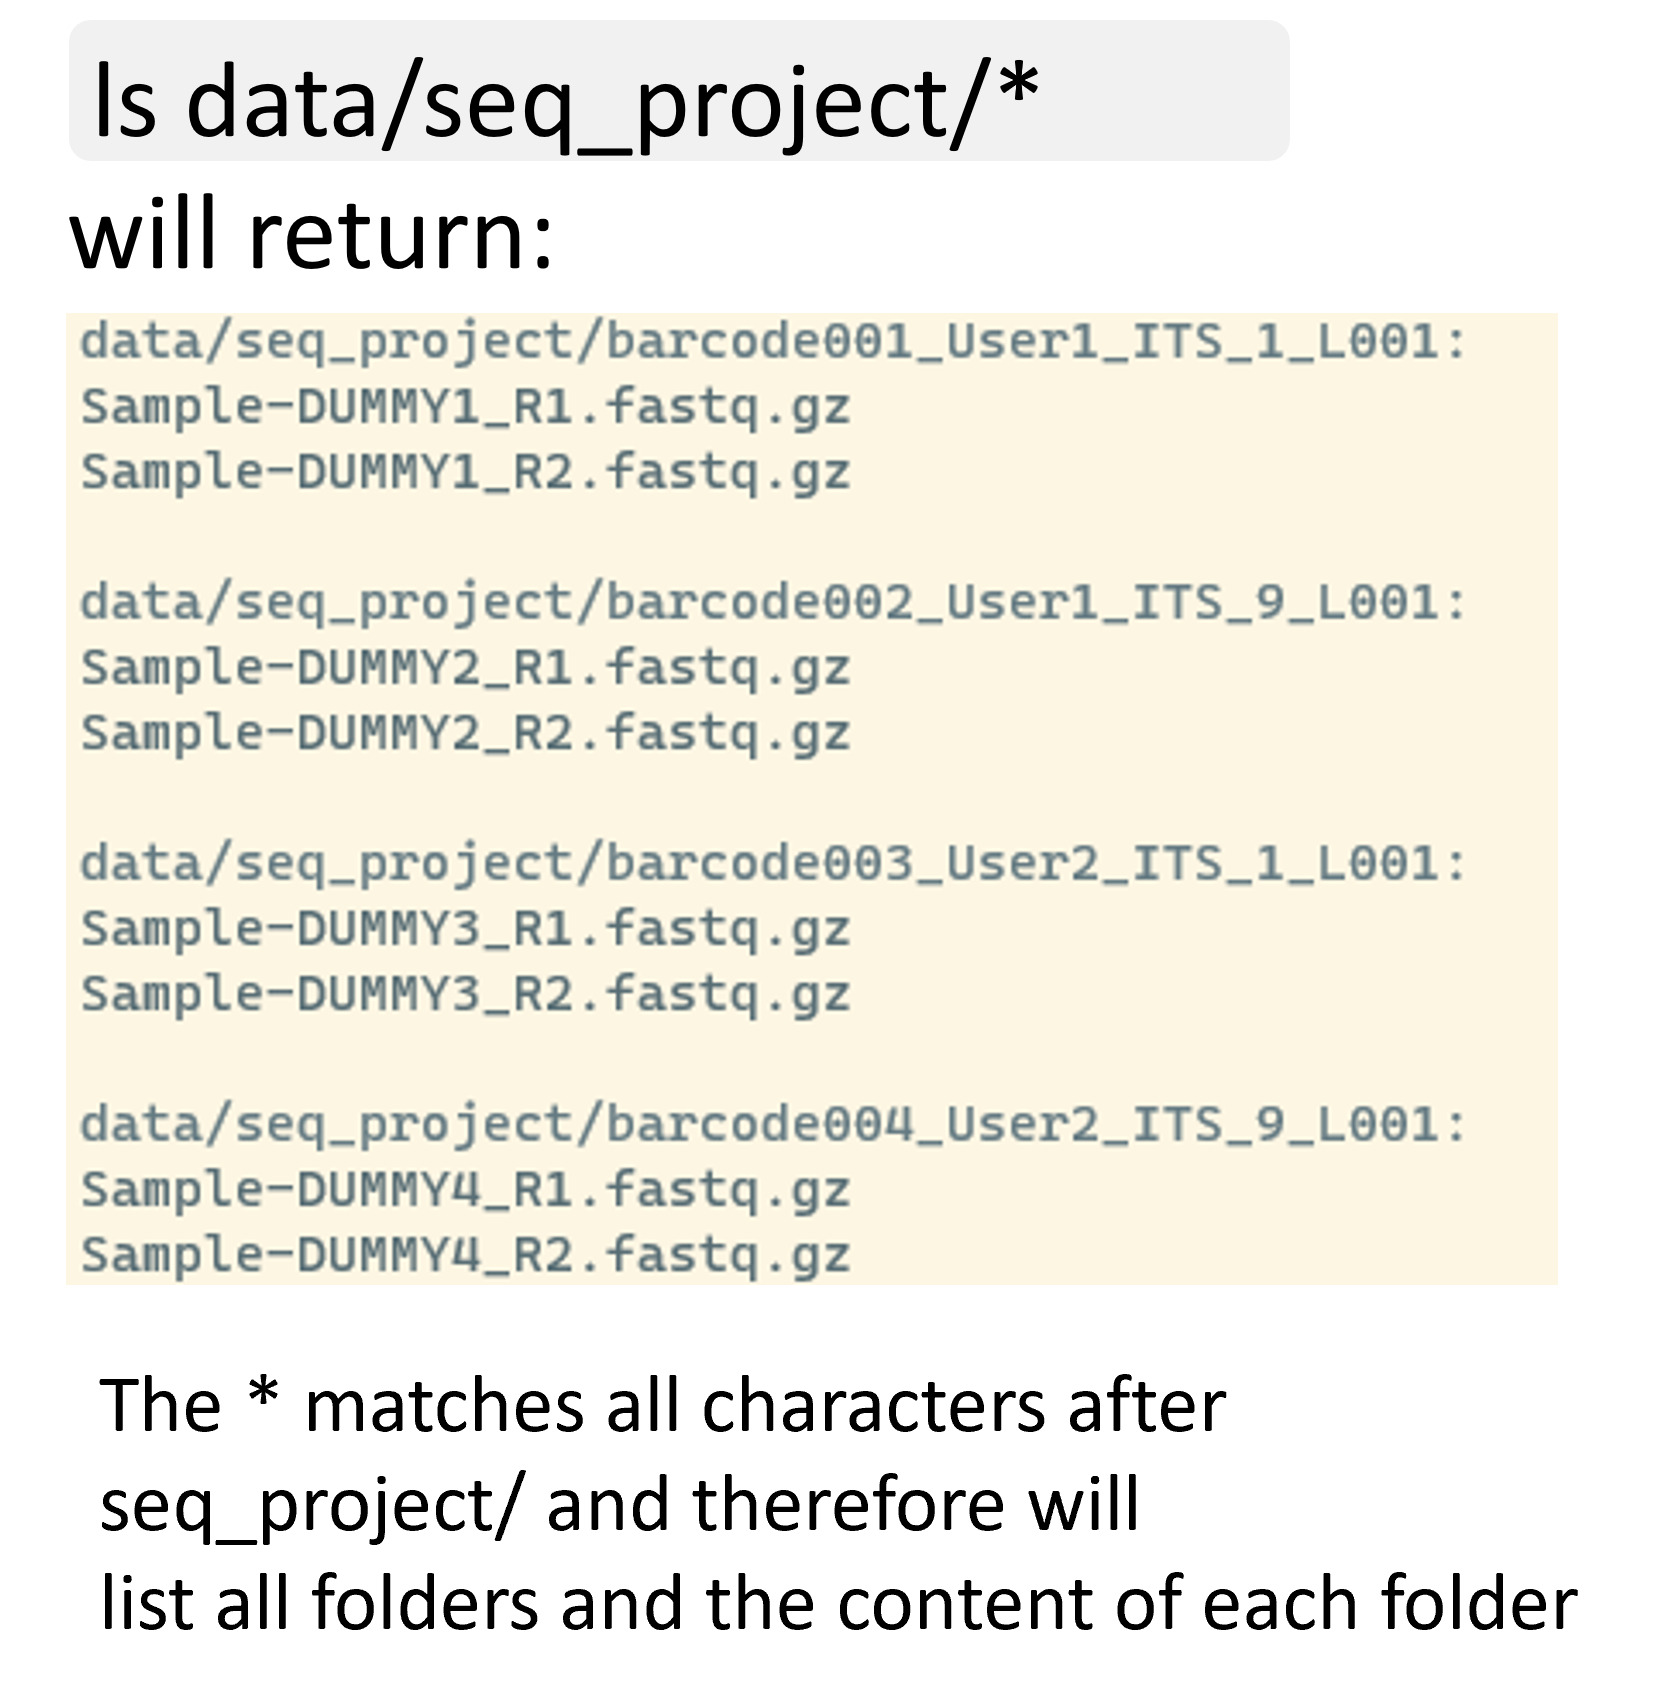
\includegraphics[width=3.28125in,height=\textheight]{../img/wildcards_0.png}

You should have seen before that the sequencing files all end with
\texttt{.fastq.gz} we can make this command a bit more specific and at
the same time make the output a bit more readable:

\begin{Shaded}
\begin{Highlighting}[]
\FunctionTok{ls}\NormalTok{ data/seq\_project/}\PreprocessorTok{*}\NormalTok{/}\PreprocessorTok{*}\NormalTok{.gz}
\end{Highlighting}
\end{Shaded}

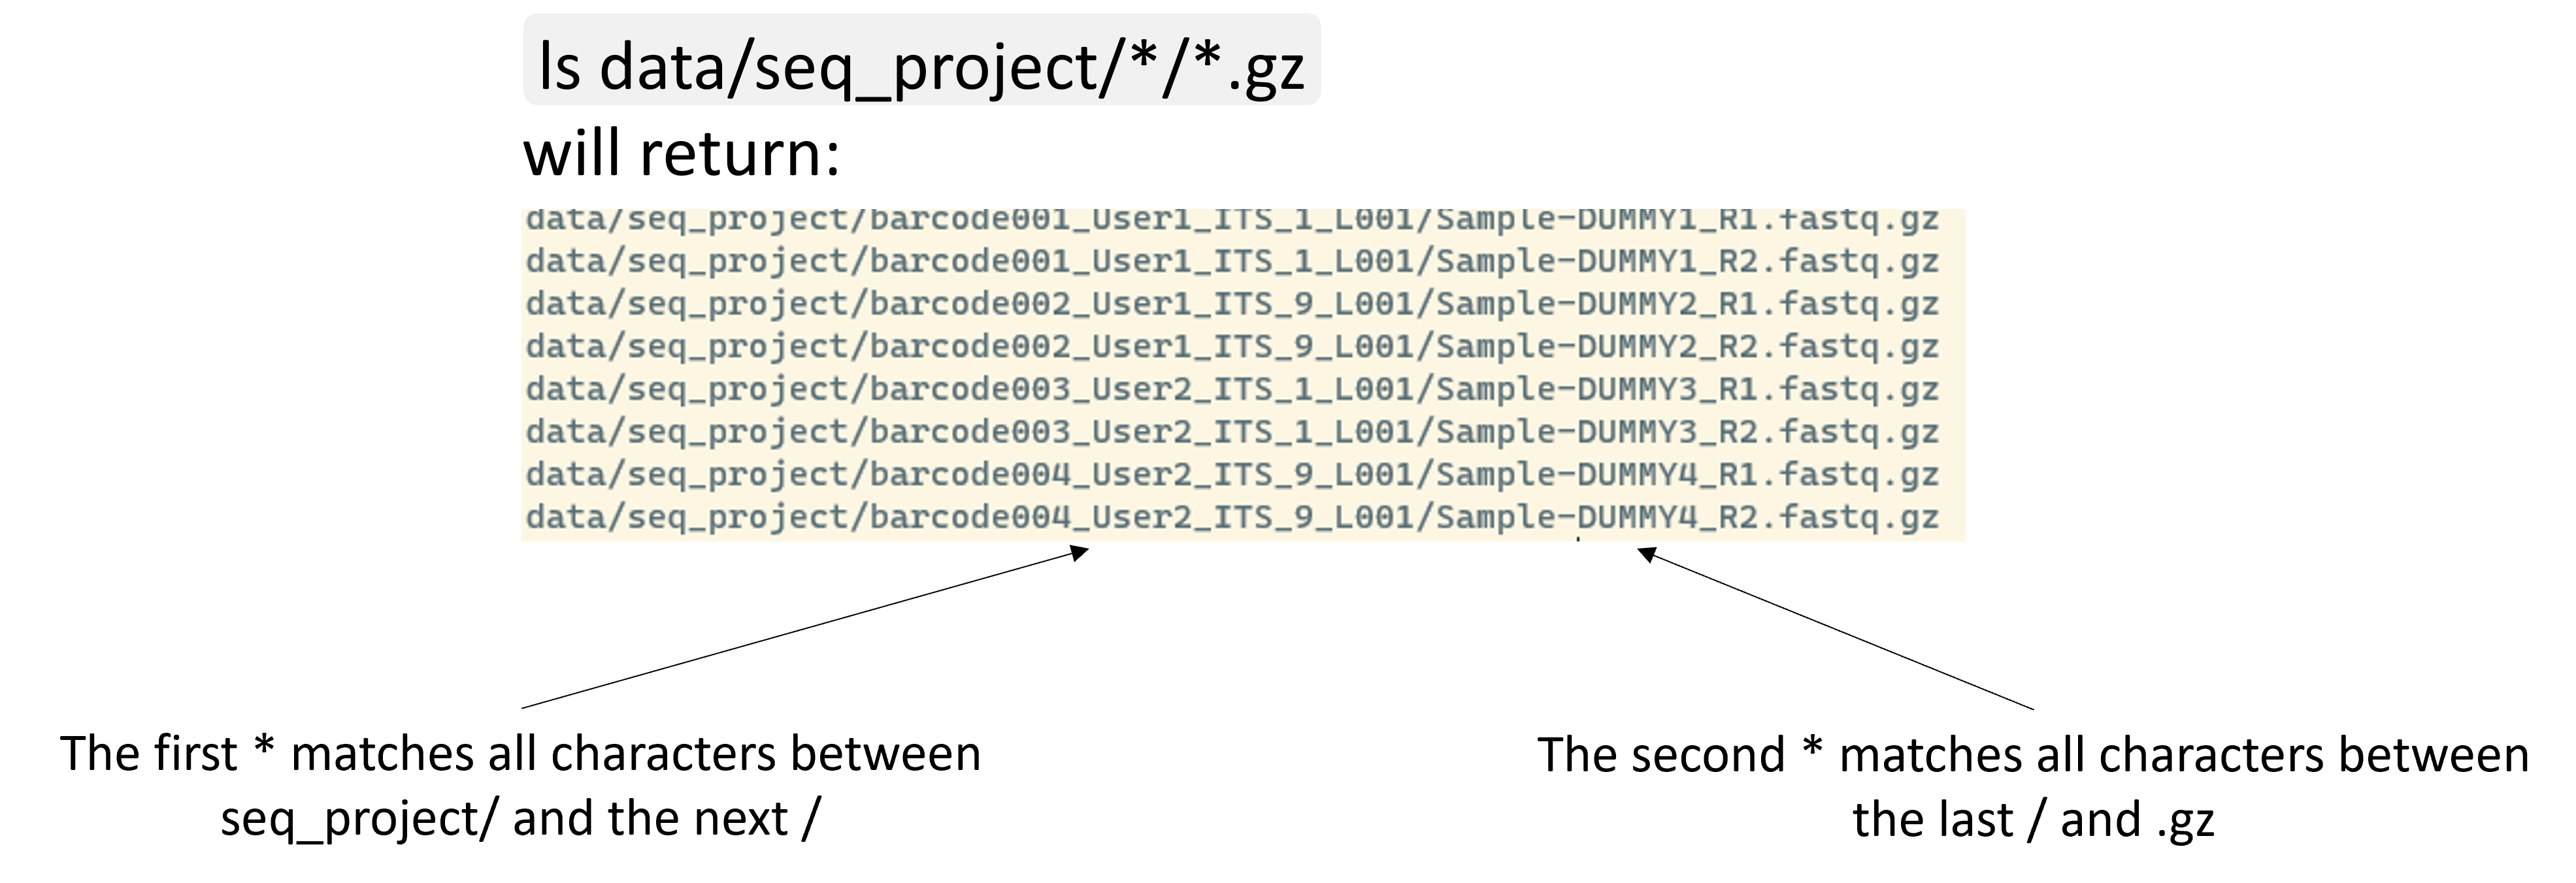
\includegraphics[width=5.8125in,height=\textheight]{../img/wildcards_1.png}

If we wanted to print the absolute and not the relative path, we could
do the following (beware that the absolute path will be slightly
different depending in you system):

\begin{Shaded}
\begin{Highlighting}[]
\FunctionTok{ls}\NormalTok{ /home/User\_name/data/seq\_project/}\PreprocessorTok{*}\NormalTok{/}\PreprocessorTok{*}\NormalTok{.gz}
\end{Highlighting}
\end{Shaded}

Now we can easily see for each folder how many files we have.

\begin{tcolorbox}[enhanced jigsaw, title=\textcolor{quarto-callout-caution-color}{\faFire}\hspace{0.5em}{Exercise}, colframe=quarto-callout-caution-color-frame, opacitybacktitle=0.6, rightrule=.15mm, arc=.35mm, left=2mm, colbacktitle=quarto-callout-caution-color!10!white, bottomrule=.15mm, leftrule=.75mm, toprule=.15mm, opacityback=0, bottomtitle=1mm, colback=white, toptitle=1mm, breakable, titlerule=0mm, coltitle=black]

\begin{enumerate}
\def\labelenumi{\arabic{enumi}.}
\tightlist
\item
  Use a wildcard to list files for barcode001 only
\item
  Use a wildcard to only list R1 (i.e.~forward) files
\item
  Use a wildcard to copy all R1 files into a new folder, call this new
  folder \texttt{R1\_files}. Use \texttt{ls} to confirm if you copied
  the right files
\item
  To avoid duplicates, remove the R1\_files folder from question 3 after
  you have ensured the command you used worked
\end{enumerate}

Click me to see an answer

\begin{Shaded}
\begin{Highlighting}[]
\CommentTok{\#question 1:}
\FunctionTok{ls}\NormalTok{ data/seq\_project/barcode001}\PreprocessorTok{*}\NormalTok{/}\PreprocessorTok{*}\NormalTok{gz}

\CommentTok{\#question 2:}
\FunctionTok{ls}\NormalTok{ data/seq\_project/}\PreprocessorTok{*}\NormalTok{/}\PreprocessorTok{*}\NormalTok{R1}\PreprocessorTok{*}

\CommentTok{\#question 3:}
\FunctionTok{mkdir}\NormalTok{ R1\_files}
\FunctionTok{cp}\NormalTok{ data/seq\_project/}\PreprocessorTok{*}\NormalTok{/}\PreprocessorTok{*}\NormalTok{R1}\PreprocessorTok{*}\NormalTok{ R1\_files}
\FunctionTok{ls}\NormalTok{ data/seq\_project/}\PreprocessorTok{*}\NormalTok{/}\PreprocessorTok{*}\NormalTok{.gz}
\FunctionTok{ls} \AttributeTok{{-}l}\NormalTok{ R1\_files}

\CommentTok{\#question 4:}
\FunctionTok{rm} \AttributeTok{{-}r}\NormalTok{ R1\_files}
\end{Highlighting}
\end{Shaded}

After solving question 2 you should see:

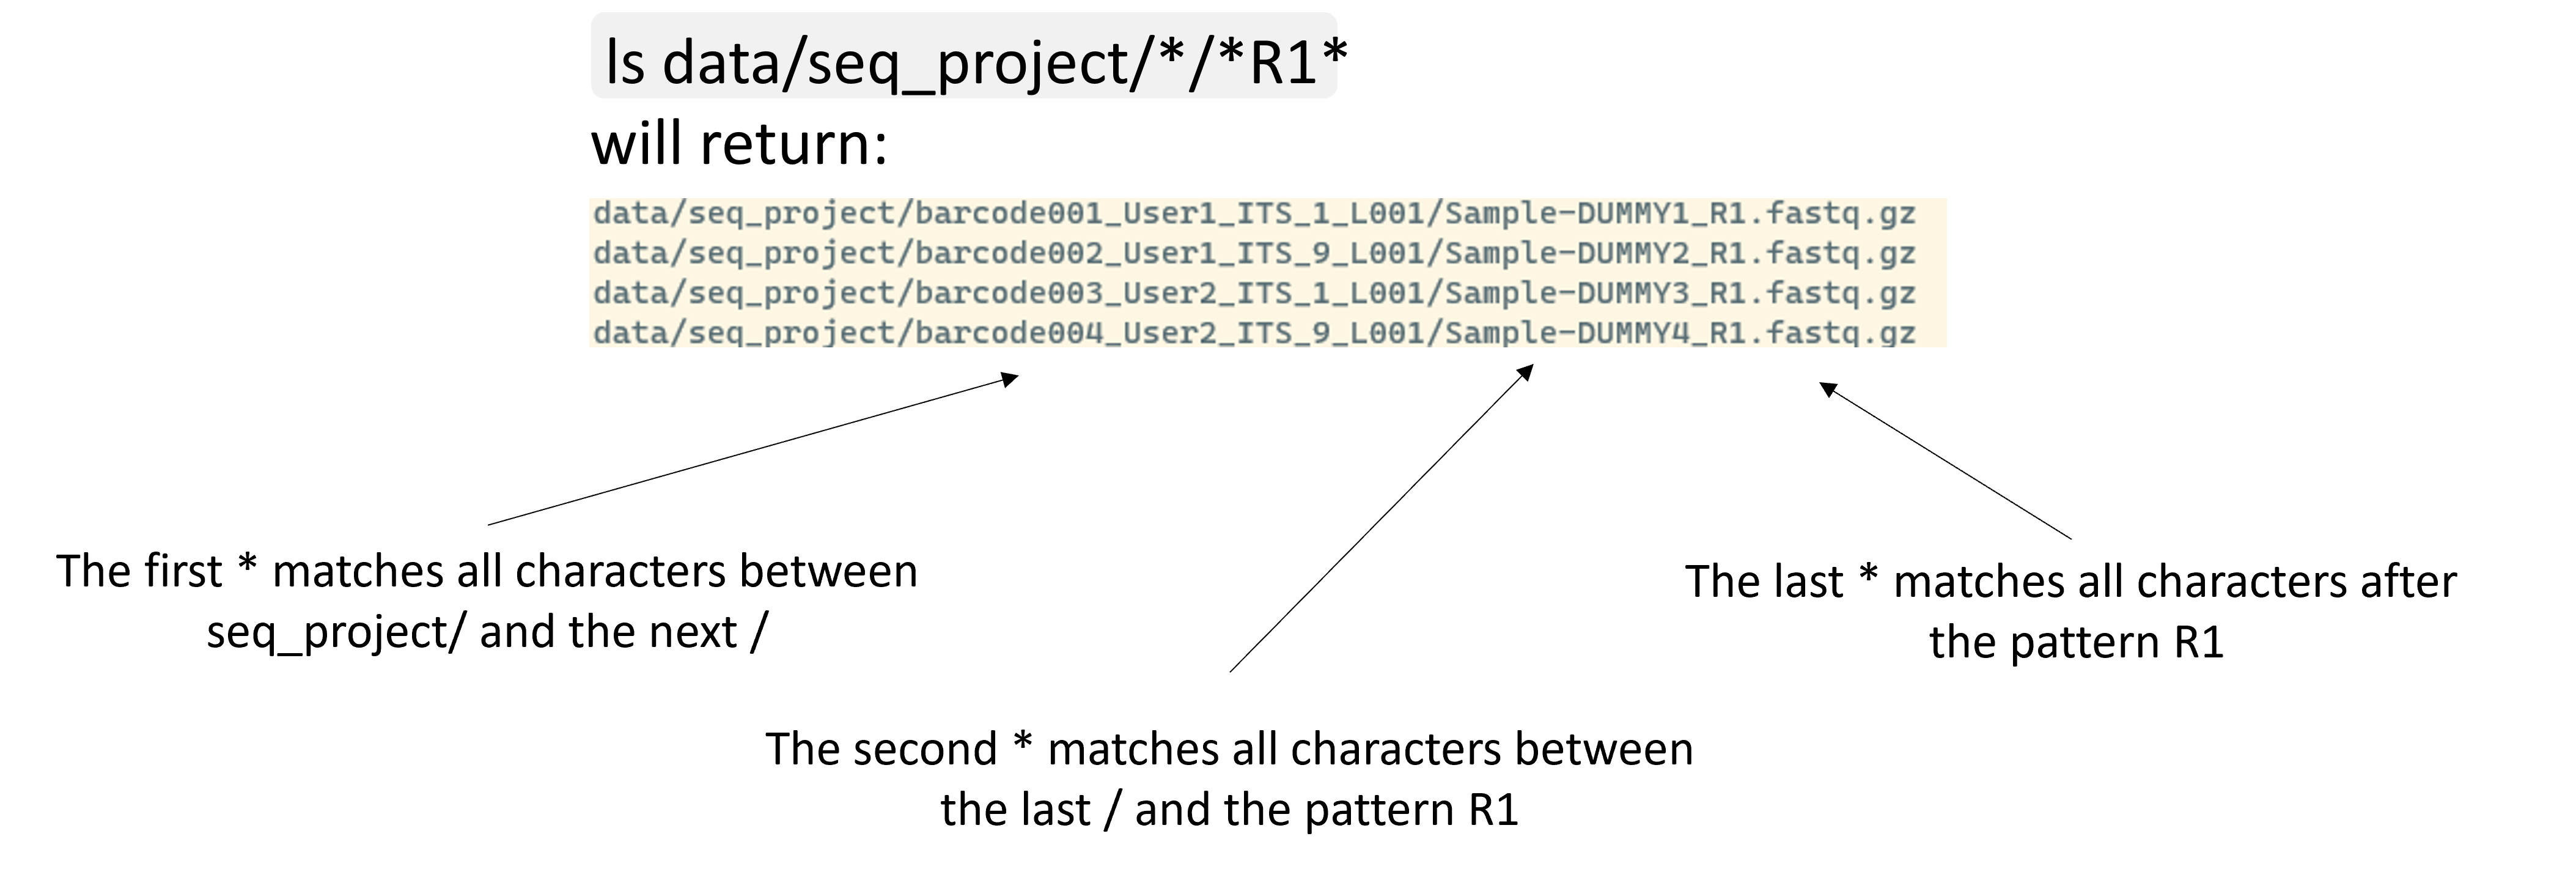
\includegraphics[width=5.09375in,height=\textheight]{../img/wildcards_3.png}

After solving question 3, we should see that all files still exist in
its original location but are now also inside of the \texttt{R1\_files}
folder. Notice, how we can use wildcards together with other commands to
easily reorganize our data?

\end{tcolorbox}

\begin{tcolorbox}[enhanced jigsaw, title=\textcolor{quarto-callout-tip-color}{\faLightbulb}\hspace{0.5em}{Tip: More wildcards}, colframe=quarto-callout-tip-color-frame, opacitybacktitle=0.6, rightrule=.15mm, arc=.35mm, left=2mm, colbacktitle=quarto-callout-tip-color!10!white, bottomrule=.15mm, leftrule=.75mm, toprule=.15mm, opacityback=0, bottomtitle=1mm, colback=white, toptitle=1mm, breakable, titlerule=0mm, coltitle=black]

\texttt{*} is not the only wildcard we can use and a full list can be
found
\href{https://tldp.org/LDP/GNU-Linux-Tools-Summary/html/x11655.htm}{here}.

Different wildcards can be useful in different contexts, not only only
when listing files but also finding patterns in files. To make such
searches as specific as possible there are different wildcards
available. A few examples are:

The {[}0-9{]} wildcard = matches any number exactly once and allows us
to extract a range of files.

\begin{Shaded}
\begin{Highlighting}[]
\FunctionTok{ls}\NormalTok{ data/seq\_project/barcode00}\PreprocessorTok{[}\SpecialStringTok{0}\PreprocessorTok{{-}}\SpecialStringTok{9}\PreprocessorTok{]*}\NormalTok{/}\PreprocessorTok{*}\NormalTok{.gz}
\end{Highlighting}
\end{Shaded}

The {[}012{]} wildcard = matches 1 or 2 exactly once and allows us to
extract a range of files.

\begin{Shaded}
\begin{Highlighting}[]
\FunctionTok{ls}\NormalTok{ data/seq\_project/barcode00}\PreprocessorTok{[}\SpecialStringTok{12}\PreprocessorTok{]*}\NormalTok{/}\PreprocessorTok{*}\NormalTok{.gz}
\end{Highlighting}
\end{Shaded}

{[}A-Z{]} matches any letter in capitals occurring once

{[}a-z{]}* matches any letter in non-capital letters occurring many
times

\begin{Shaded}
\begin{Highlighting}[]
\FunctionTok{ls}\NormalTok{ data/seq\_project/barcode001\_User1\_ITS\_1\_}\PreprocessorTok{[}\SpecialStringTok{A}\PreprocessorTok{{-}}\SpecialStringTok{Z}\PreprocessorTok{]}\NormalTok{001/}\PreprocessorTok{*}\NormalTok{.gz}
\end{Highlighting}
\end{Shaded}

\end{tcolorbox}

\section{I/O redirection to new
files}\label{io-redirection-to-new-files}

We have seen that by default our commands directly print the standard
output to the terminal. For example, when we use \texttt{ls} the list of
files and folders is printed to your terminal. However, we can also
redirect the standard output to a file by using the
\texttt{\textgreater{}} character.

For example, we might want to generate a list with all fastq files and
can do this as follows:

\begin{Shaded}
\begin{Highlighting}[]
\FunctionTok{ls}\NormalTok{ data/seq\_project/}\PreprocessorTok{*}\NormalTok{/}\PreprocessorTok{*} \OperatorTok{\textgreater{}}\NormalTok{ fastq\_paths.txt}
\end{Highlighting}
\end{Shaded}

\section{Exploring the content of text
files}\label{exploring-the-content-of-text-files}

Next, let's view the content of the list we just generated. Viewing the
actual files we work with is often important to ensure the integrity of
our data.

\subsubsection{\texorpdfstring{\texttt{head}: View the first rows of a
file}{head: View the first rows of a file}}\label{head-view-the-first-rows-of-a-file}

\texttt{head} can be used to check the first 10 rows of our files:

\begin{Shaded}
\begin{Highlighting}[]
\FunctionTok{head}\NormalTok{ fastq\_paths.txt}
\end{Highlighting}
\end{Shaded}

\subsection{\texorpdfstring{\texttt{tail}: View the last rows of a
file}{tail: View the last rows of a file}}\label{tail-view-the-last-rows-of-a-file}

If you want to check the last 10 rows use \texttt{tail}:

\begin{Shaded}
\begin{Highlighting}[]
\FunctionTok{tail}\NormalTok{ fastq\_paths.txt}
\end{Highlighting}
\end{Shaded}

\subsection{\texorpdfstring{\texttt{less}: View the full
file}{less: View the full file}}\label{less-view-the-full-file}

\texttt{less} is a program that let's you view a file's contents one
screen at a time. This is useful when dealing with a large text file
(such as a sequence data file) because it doesn't load the entire file
but accesses it page by page, resulting in fast loading speeds.

\begin{Shaded}
\begin{Highlighting}[]
\FunctionTok{less} \AttributeTok{{-}S}\NormalTok{ fastq\_paths.txt}
\end{Highlighting}
\end{Shaded}

\begin{itemize}
\tightlist
\item
  You can use the arrow Up and Page arrow keys to move through the text
  file
\item
  To exit less, type \texttt{q}
\end{itemize}

\begin{tcolorbox}[enhanced jigsaw, title=\textcolor{quarto-callout-tip-color}{\faLightbulb}\hspace{0.5em}{Tip: Editing text files}, colframe=quarto-callout-tip-color-frame, opacitybacktitle=0.6, rightrule=.15mm, arc=.35mm, left=2mm, colbacktitle=quarto-callout-tip-color!10!white, bottomrule=.15mm, leftrule=.75mm, toprule=.15mm, opacityback=0, bottomtitle=1mm, colback=white, toptitle=1mm, breakable, titlerule=0mm, coltitle=black]

You can also edit the content of a text file and there are different
programs available to do this on the command line, the most commonly
used tool is \texttt{nano}, which should come with most command line
interpreters. You can open any file as follows:

\begin{Shaded}
\begin{Highlighting}[]
\FunctionTok{nano}\NormalTok{ fastq\_paths.txt}
\end{Highlighting}
\end{Shaded}

Once the document is open you can edit it however you want and then

\begin{itemize}
\tightlist
\item
  Close the document with \texttt{control\ +\ X}
\item
  Type \texttt{y} to save changes and press enter
\end{itemize}

\end{tcolorbox}

\section{\texorpdfstring{\texttt{wc}: Count
things}{wc: Count things}}\label{wc-count-things}

Another useful tool is the \texttt{wc} (= wordcount) command that allows
us to count the number of lines via \texttt{-l} in a file. It is an
useful tool for sanity checking and here allows us to count how many
files we work with:

\begin{Shaded}
\begin{Highlighting}[]
\FunctionTok{wc} \AttributeTok{{-}l}\NormalTok{ fastq\_paths.txt}
\end{Highlighting}
\end{Shaded}

After running this we see that we work with 8 files.

We could of course easily count this ourselves, however, if we work with
hundreds of files its a quick and easy way to get an overview about how
much data we work with.

One down-side of this approach is that to be able to count the number of
files, we first need to generate a file in which we count the number of
files. This (i) can create files we do not actually need and (ii) we use
two commands while ideally we want to get the information with a single
command.

\section{Pipes}\label{pipes}

Pipes are a powerful utility to connect multiple commands together.
Pipes allow us to feed the standard output of one command, such as
\texttt{ls} as input into another command, such as \texttt{wc\ -l}, and
as such combine multiple commands together.

Therefore, let`s use \texttt{ls} to first list all fastq files and then
pipe the output from \texttt{ls} into the \texttt{wc} command in order
to count with how many files we work with:

\begin{Shaded}
\begin{Highlighting}[]
\FunctionTok{ls}\NormalTok{ data/seq\_project/}\PreprocessorTok{*}\NormalTok{/}\PreprocessorTok{*} \KeywordTok{|} \FunctionTok{wc} \AttributeTok{{-}l}
\end{Highlighting}
\end{Shaded}

We should see again that we work with 8 files, but now we did not have
to generate an intermediate text file and have a more condensed command.

\begin{tcolorbox}[enhanced jigsaw, title=\textcolor{quarto-callout-caution-color}{\faFire}\hspace{0.5em}{Exercise}, colframe=quarto-callout-caution-color-frame, opacitybacktitle=0.6, rightrule=.15mm, arc=.35mm, left=2mm, colbacktitle=quarto-callout-caution-color!10!white, bottomrule=.15mm, leftrule=.75mm, toprule=.15mm, opacityback=0, bottomtitle=1mm, colback=white, toptitle=1mm, breakable, titlerule=0mm, coltitle=black]

\begin{enumerate}
\def\labelenumi{\arabic{enumi}.}
\tightlist
\item
  Use ls and wc to count how many R1 files we have
\item
  Count how many R2 files we have
\item
  Count how many files were generated for User1
\end{enumerate}

Click me to see an answer

\begin{Shaded}
\begin{Highlighting}[]
\CommentTok{\#question 1: We see 4 files}
\FunctionTok{ls}\NormalTok{ data/seq\_project/}\PreprocessorTok{*}\NormalTok{/}\PreprocessorTok{*}\NormalTok{R1}\PreprocessorTok{*}\NormalTok{gz }\KeywordTok{|} \FunctionTok{wc} \AttributeTok{{-}l} 

\CommentTok{\#question 2: We see 4 files}
\FunctionTok{ls}\NormalTok{ data/seq\_project/}\PreprocessorTok{*}\NormalTok{/}\PreprocessorTok{*}\NormalTok{R2}\PreprocessorTok{*}\NormalTok{gz }\KeywordTok{|} \FunctionTok{wc} \AttributeTok{{-}l} 

\CommentTok{\#question 3: We see 4 files}
\FunctionTok{ls}\NormalTok{ data/seq\_project/}\PreprocessorTok{*}\NormalTok{\_User1\_}\PreprocessorTok{*}\NormalTok{/}\PreprocessorTok{*}\NormalTok{gz }\KeywordTok{|} \FunctionTok{wc} \AttributeTok{{-}l} 
\end{Highlighting}
\end{Shaded}

Checking whether we have the same number of R1 and R2 files is a good
sanity check, to ensure that we have received all the files from the
sequencing center whenever we generate paired-end sequencing data.

\end{tcolorbox}

\section{\texorpdfstring{\texttt{cut}: Extract elements from
strings}{cut: Extract elements from strings}}\label{cut-extract-elements-from-strings}

Remember, how we stored a list of sequencing files and the path leading
to these files (relative to our home directory in a text file called
\texttt{fastq\_paths.txt})?

Imagine that we only wanted to have a list of files but not the path,
how would we do that?

There are different ways to do this, the simplest one is to use
\texttt{cd} and go into the folder with our sequence files and generate
a list in there.

However, another way in which we do not have move around (and learn some
other concepts) is to use the \texttt{cut} command. \texttt{cut} allows
us to separate lines of text into different elements using any kind of
delimiter, for example the \texttt{/} that we use in the file path. To
ensure that \texttt{/} is seen a separator we use the \texttt{-d} option
and with \texttt{-f4} we tell cut to print the fourth element of each
separated field.

\begin{Shaded}
\begin{Highlighting}[]
\FunctionTok{head}\NormalTok{ fastq\_paths.txt}

\CommentTok{\#extract the file name (i.e. the fourth field when using a / separator)}
\FunctionTok{cut} \AttributeTok{{-}f4} \AttributeTok{{-}d} \StringTok{"/"}\NormalTok{ fastq\_paths.txt}

\CommentTok{\#do the same as above but this time save the output in a new file}
\FunctionTok{cut} \AttributeTok{{-}f4} \AttributeTok{{-}d} \StringTok{"/"}\NormalTok{ fastq\_paths.txt }\OperatorTok{\textgreater{}}\NormalTok{ fastq\_files.txt}
\end{Highlighting}
\end{Shaded}

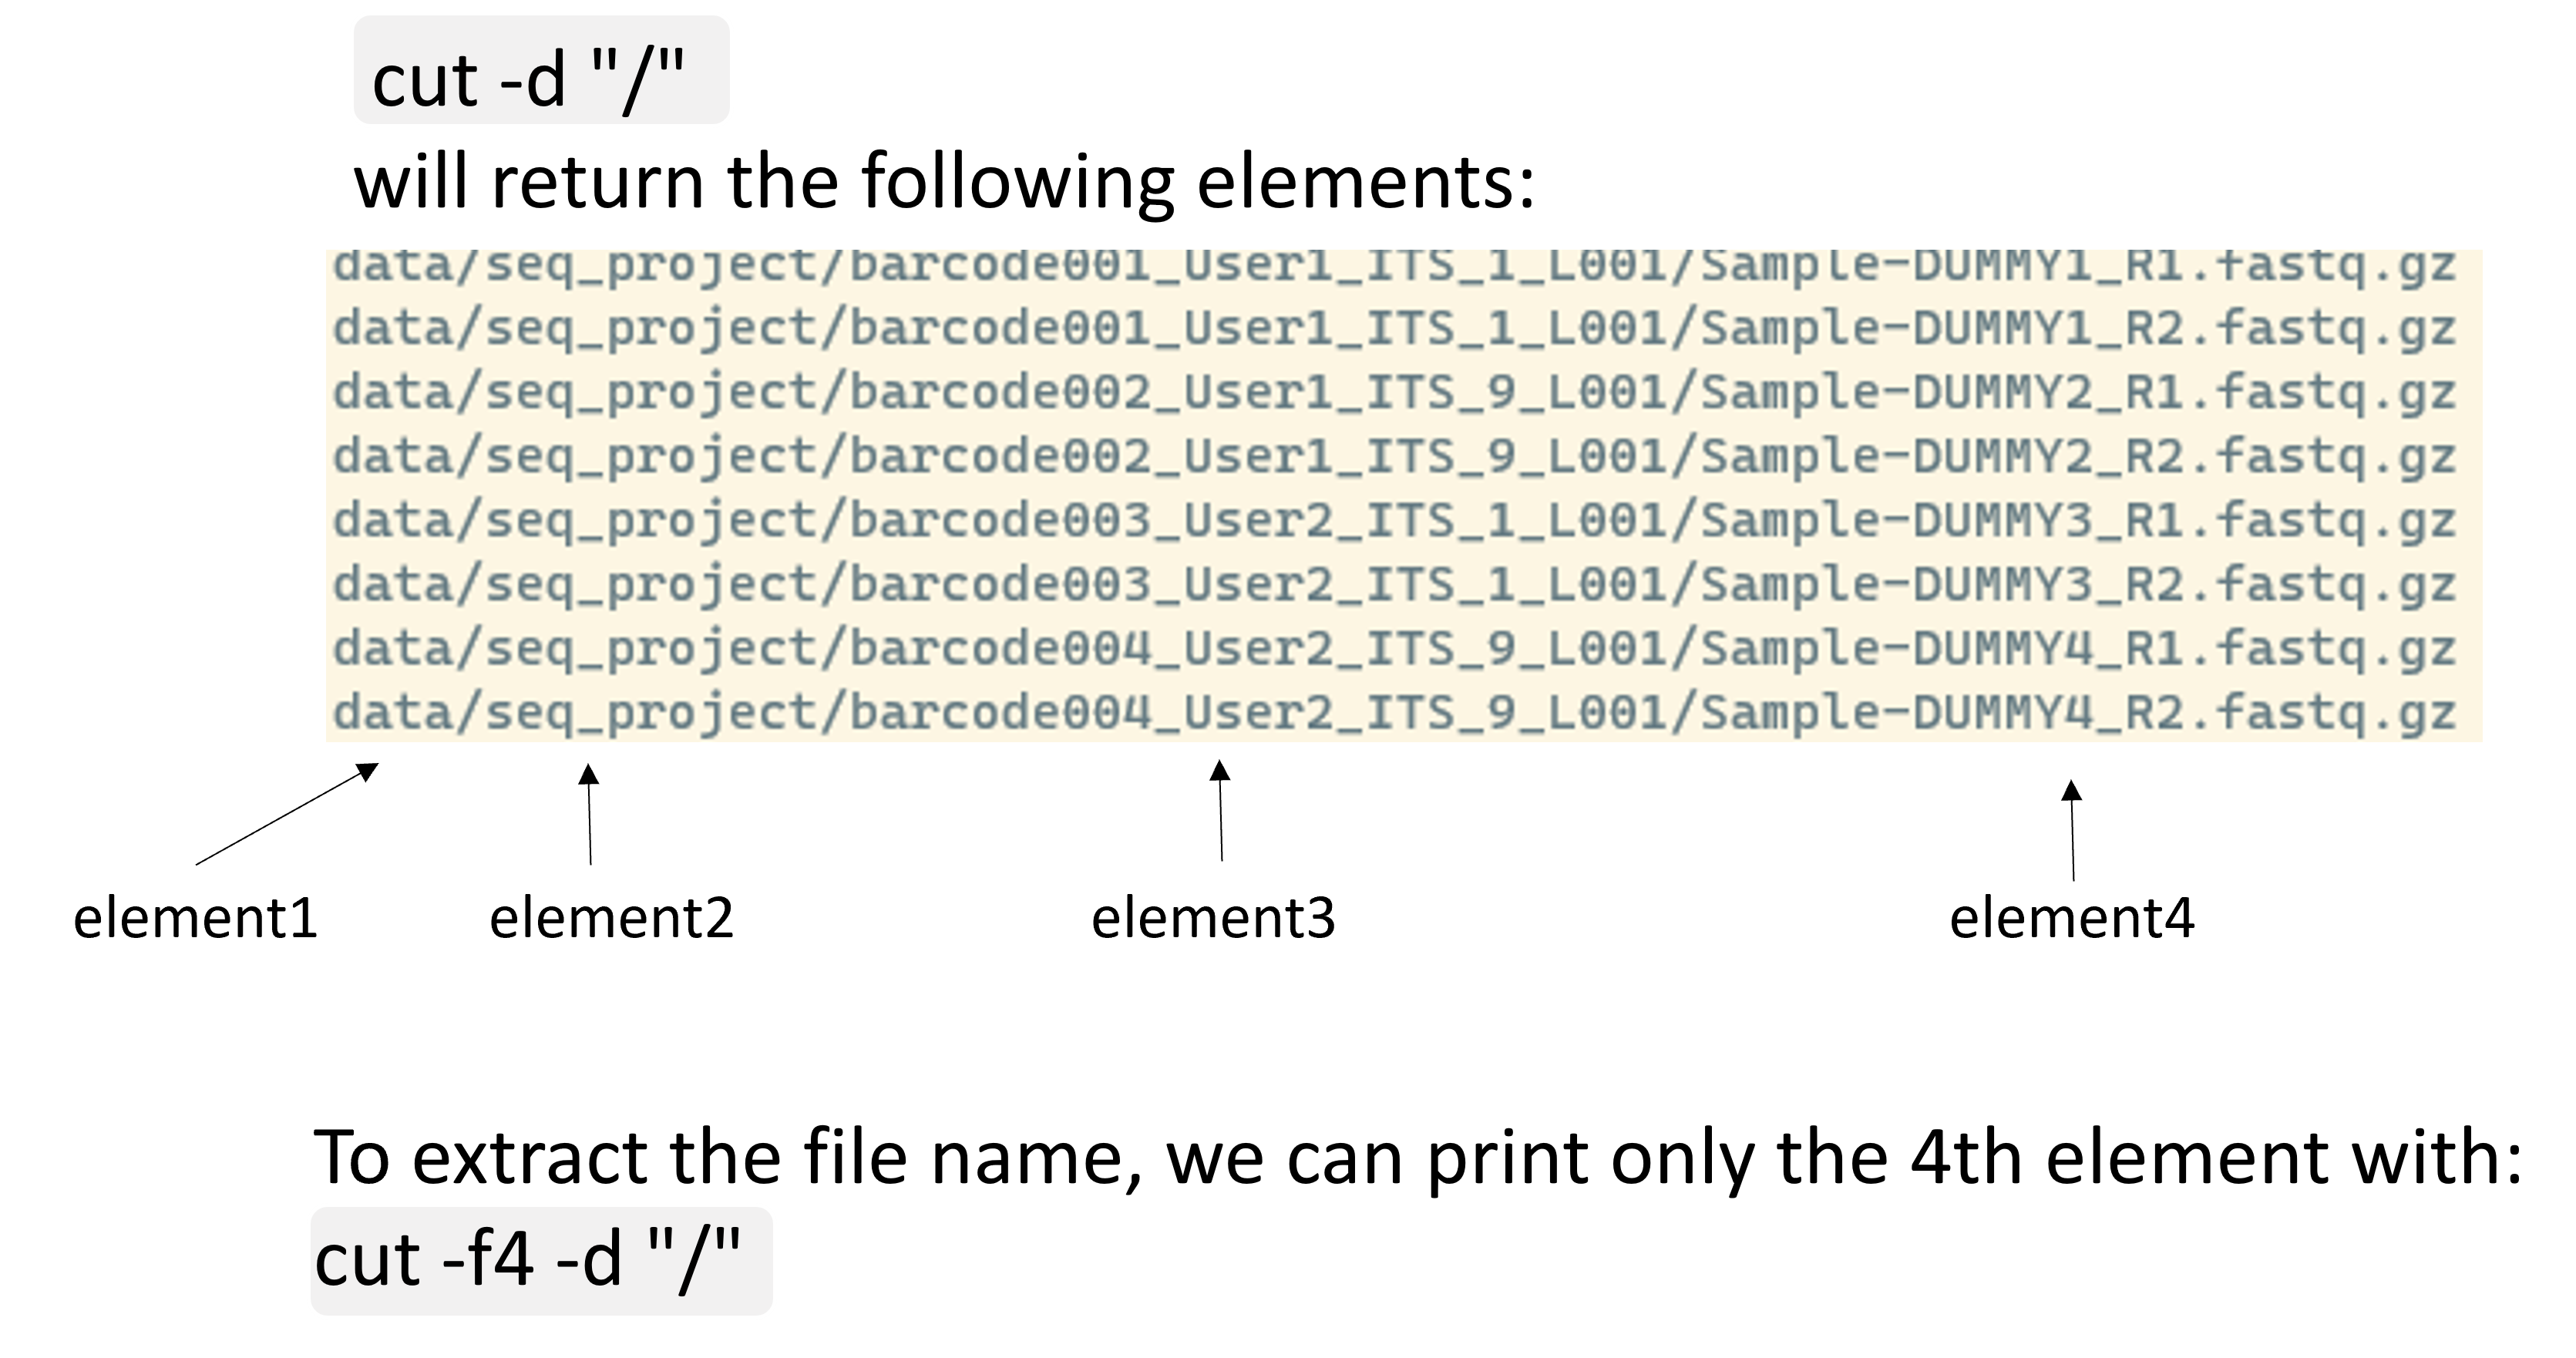
\includegraphics[width=4.80208in,height=\textheight]{../img/cut_1.pnd.png}

We can also combine this with pipes in order to extract different pieces
of information. Let's assume we start with extracting a folder name,
such as \texttt{barcode002\_User1\_ITS\_9\_L001}, and from that we want
to extract some other information, such as the barcode IDs. We can
easily do this as follows:

\begin{Shaded}
\begin{Highlighting}[]
\FunctionTok{cut} \AttributeTok{{-}f3} \AttributeTok{{-}d} \StringTok{"/"}\NormalTok{ fastq\_paths.txt }\KeywordTok{|} \FunctionTok{cut} \AttributeTok{{-}f1} \AttributeTok{{-}d} \StringTok{"\_"}
\end{Highlighting}
\end{Shaded}

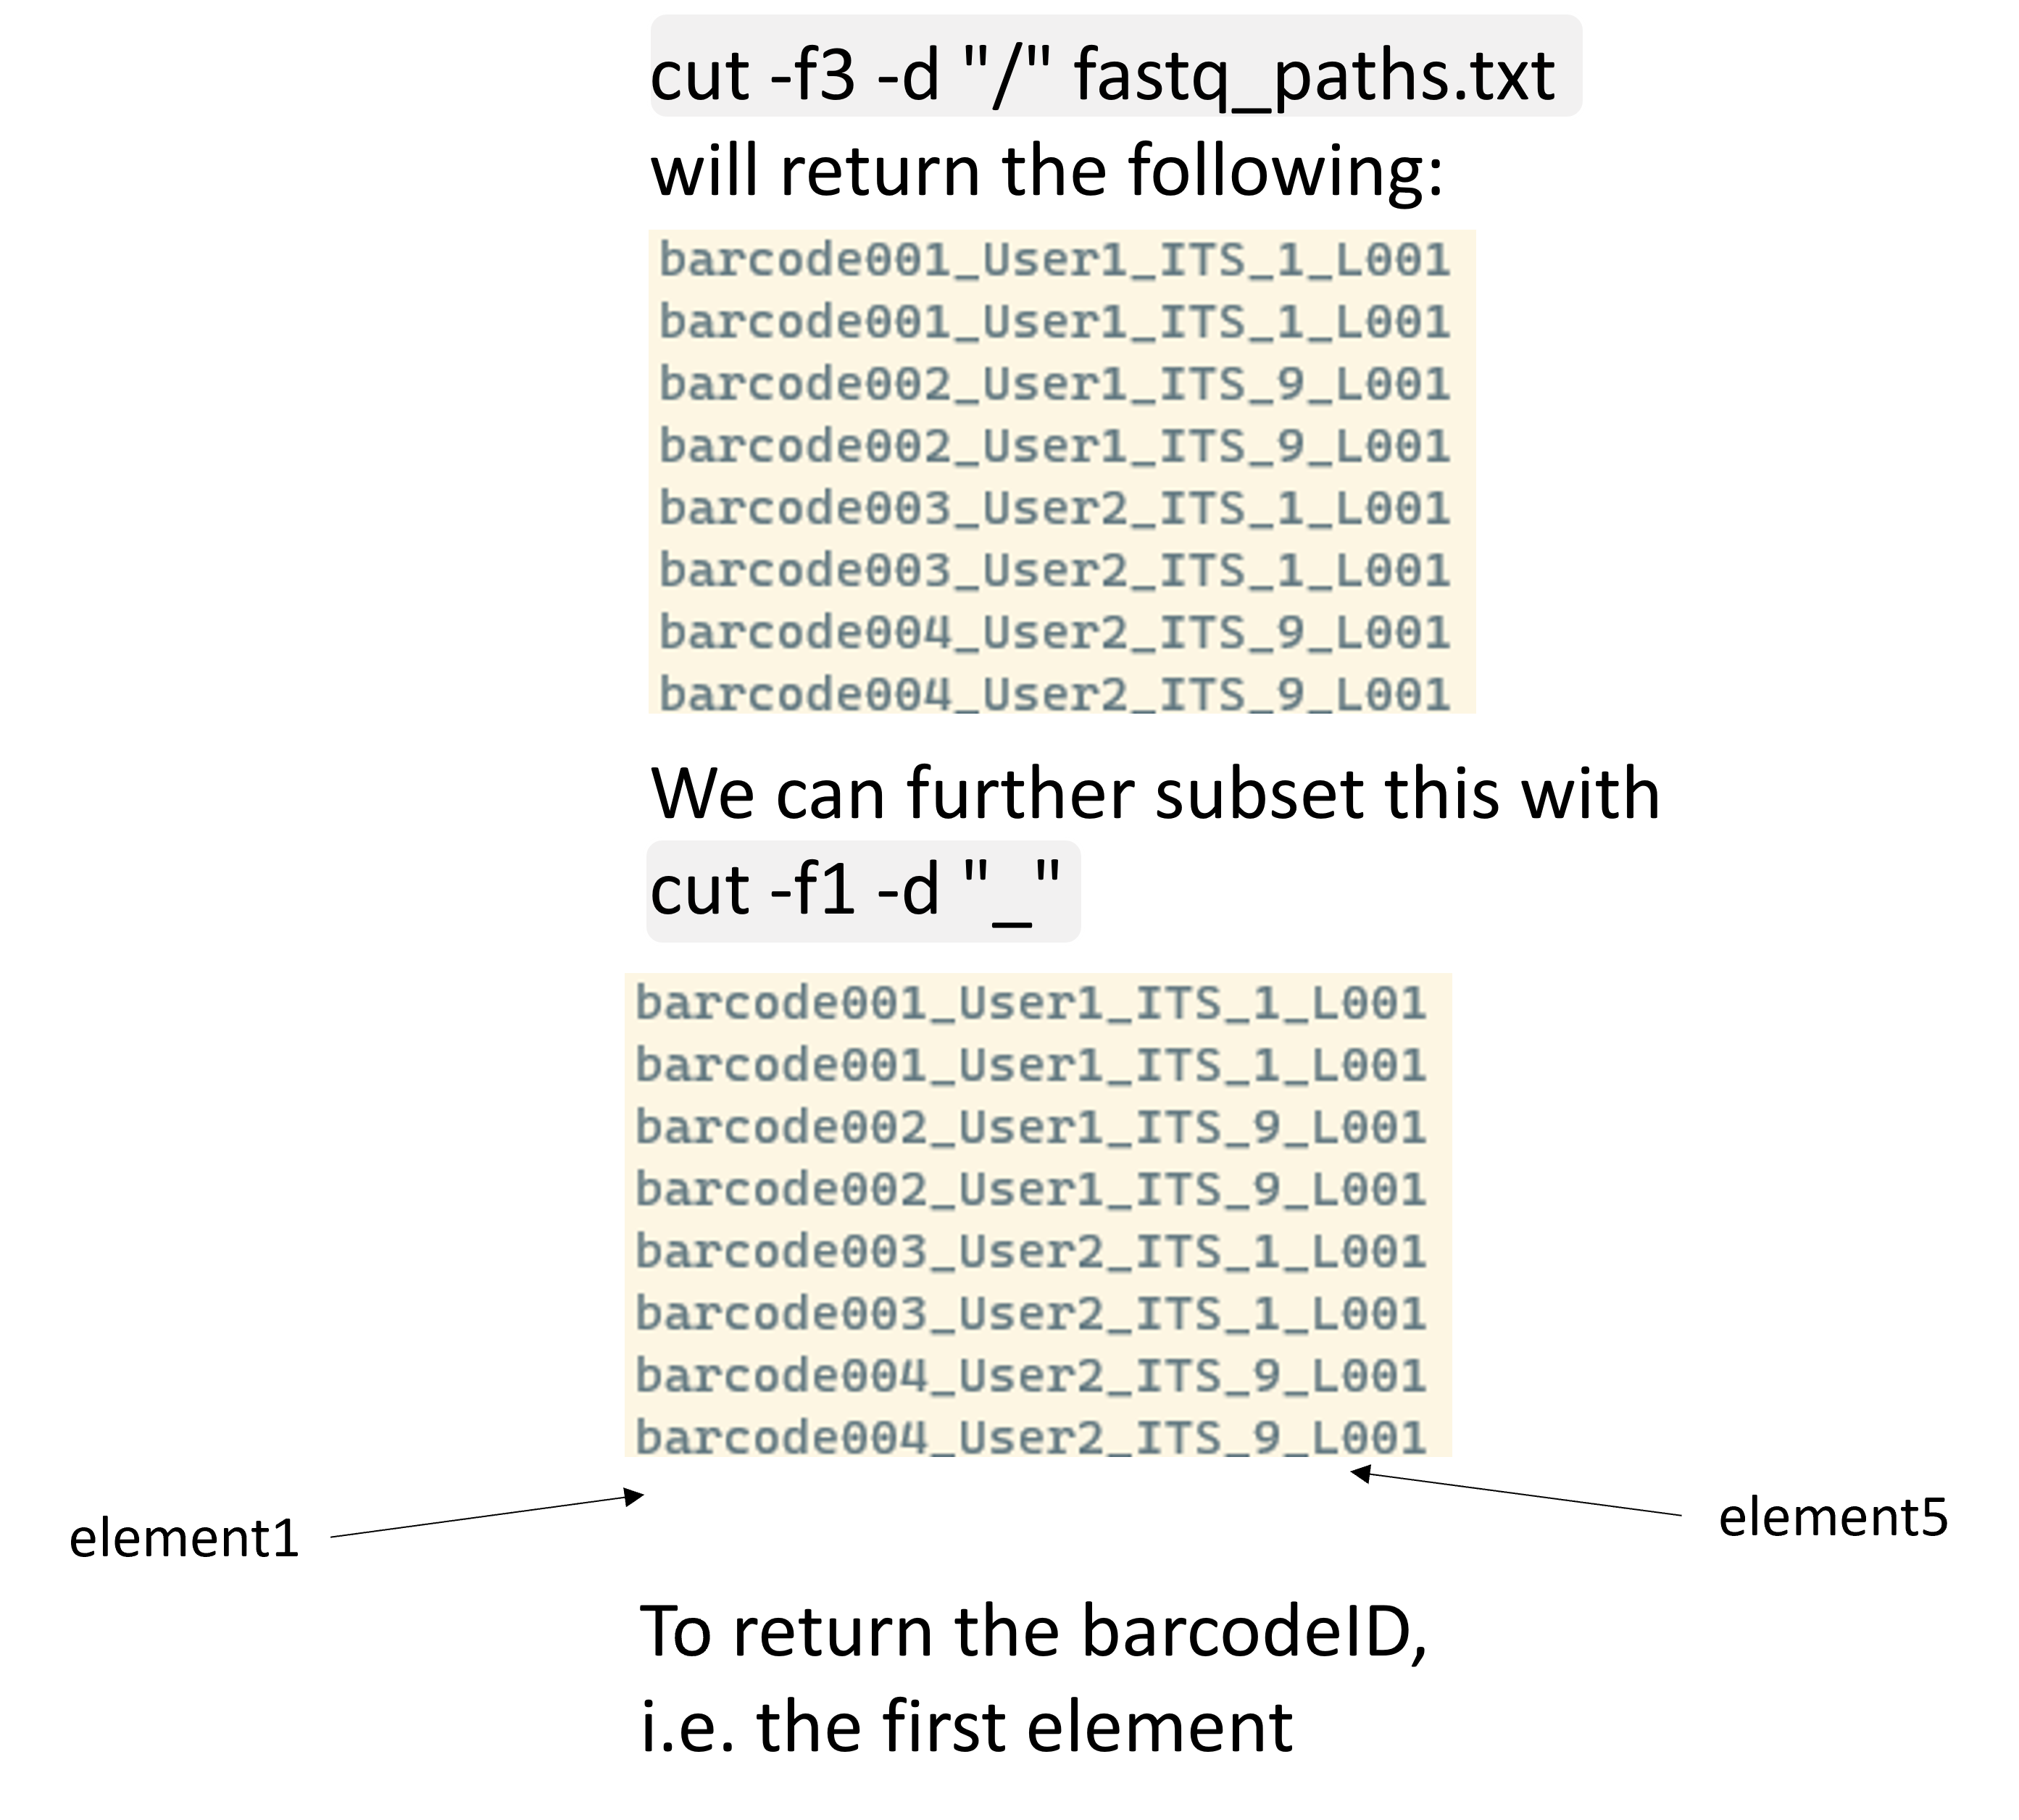
\includegraphics[width=4.04167in,height=\textheight]{../img/cut_2.png}

Nice, we now only have a list with barcodes. However, its not yet ideal
since we have duplicated barcodes. If you want to extract this
information for some metadata file this is not ideal and we need to get
to know two more commands to make this work:

\section{\texorpdfstring{\texttt{sort} and \texttt{uniq}: Create unique
lists}{sort and uniq: Create unique lists}}\label{sort-and-uniq-create-unique-lists}

\begin{itemize}
\tightlist
\item
  \texttt{sort}: sorts lines in a file from A-Z
\item
  \texttt{uniq}: removes or finds duplicates . For this command to work
  you need to provide it with a sorted file
\end{itemize}

Let's first ensure that our barcode list is sorted to then extract only
the unique information:

\begin{Shaded}
\begin{Highlighting}[]
\FunctionTok{cut} \AttributeTok{{-}f3} \AttributeTok{{-}d} \StringTok{"/"}\NormalTok{ fastq\_paths.txt }\KeywordTok{|} \FunctionTok{cut} \AttributeTok{{-}f1} \AttributeTok{{-}d} \StringTok{"\_"} \KeywordTok{|} \FunctionTok{sort} \KeywordTok{|} \FunctionTok{uniq}
\end{Highlighting}
\end{Shaded}

\begin{tcolorbox}[enhanced jigsaw, title=\textcolor{quarto-callout-caution-color}{\faFire}\hspace{0.5em}{Exercise}, colframe=quarto-callout-caution-color-frame, opacitybacktitle=0.6, rightrule=.15mm, arc=.35mm, left=2mm, colbacktitle=quarto-callout-caution-color!10!white, bottomrule=.15mm, leftrule=.75mm, toprule=.15mm, opacityback=0, bottomtitle=1mm, colback=white, toptitle=1mm, breakable, titlerule=0mm, coltitle=black]

\begin{enumerate}
\def\labelenumi{\arabic{enumi}.}
\tightlist
\item
  Use cut on fastq\_paths.txt to print the folder names in which the
  fastq.gz files reside (i.e.~barcode001\_User1\_ITS\_1\_L001)
\item
  Print the folder names as in 1 and then extract the user names from
  this list
\item
  Ensure that when running the code from 2 that we print a unique list
  of user names
\end{enumerate}

Click me to see an answer

\begin{Shaded}
\begin{Highlighting}[]
\CommentTok{\#question 1:}
\FunctionTok{cut} \AttributeTok{{-}f3} \AttributeTok{{-}d} \StringTok{"/"}\NormalTok{ fastq\_paths.txt}

\CommentTok{\#question 2:}
\FunctionTok{cut} \AttributeTok{{-}f3} \AttributeTok{{-}d} \StringTok{"/"}\NormalTok{ fastq\_paths.txt }\KeywordTok{|} \FunctionTok{cut} \AttributeTok{{-}f2} \AttributeTok{{-}d} \StringTok{"\_"}

\CommentTok{\#question 3:}
\FunctionTok{cut} \AttributeTok{{-}f3} \AttributeTok{{-}d} \StringTok{"/"}\NormalTok{ fastq\_paths.txt }\KeywordTok{|} \FunctionTok{cut} \AttributeTok{{-}f2} \AttributeTok{{-}d} \StringTok{"\_"} \KeywordTok{|} \FunctionTok{sort} \KeywordTok{|} \FunctionTok{uniq}
\end{Highlighting}
\end{Shaded}

\end{tcolorbox}

\section{\texorpdfstring{\texttt{cat}: Read and combine
files}{cat: Read and combine files}}\label{cat-read-and-combine-files}

\texttt{cat} can do different things:

\begin{enumerate}
\def\labelenumi{\arabic{enumi}.}
\tightlist
\item
  Create new files
\item
  Display the content of a file
\item
  Concatenate, i.e.~combine, several files. For concatenation we can
  provide \texttt{cat} with multiple file listed after each other or use
  a wildcard.
\end{enumerate}

To view files we do:

\begin{Shaded}
\begin{Highlighting}[]
\FunctionTok{cat}\NormalTok{ fastq\_paths.txt}
\end{Highlighting}
\end{Shaded}

To combine files we do:

\begin{Shaded}
\begin{Highlighting}[]
\CommentTok{\#combine files }
\FunctionTok{cat}\NormalTok{ fastq\_paths.txt fastq\_files.txt }\OperatorTok{\textgreater{}}\NormalTok{ combined\_files.txt}

\CommentTok{\#view new file }
\FunctionTok{cat}\NormalTok{ combined\_files.txt}
\end{Highlighting}
\end{Shaded}

\begin{tcolorbox}[enhanced jigsaw, title=\textcolor{quarto-callout-caution-color}{\faFire}\hspace{0.5em}{Exercise}, colframe=quarto-callout-caution-color-frame, opacitybacktitle=0.6, rightrule=.15mm, arc=.35mm, left=2mm, colbacktitle=quarto-callout-caution-color!10!white, bottomrule=.15mm, leftrule=.75mm, toprule=.15mm, opacityback=0, bottomtitle=1mm, colback=white, toptitle=1mm, breakable, titlerule=0mm, coltitle=black]

Fastq.gz files can easily be combined using \texttt{cat} and while this
is not strictly necessary in our case, you might need to do this with
your sequence files in the future. For example if you sequenced a lot of
data and for space reasons the sequencing center send you multiple files
for a single sample.

\begin{enumerate}
\def\labelenumi{\arabic{enumi}.}
\tightlist
\item
  Using wildcards and cat, combine all R1 fastq.gz files into a single
  file
\item
  Use ls to judge the file size of the individual R1 files and the
  combined file to assess whether everything worked correctly
\end{enumerate}

Click me to see an answer

\begin{Shaded}
\begin{Highlighting}[]
\CommentTok{\#question 1:}
\FunctionTok{cat}\NormalTok{ data/seq\_project/}\PreprocessorTok{*}\NormalTok{/}\PreprocessorTok{*}\NormalTok{R1.fastq.gz }\OperatorTok{\textgreater{}}\NormalTok{ combined\_R1.fastq.gz}

\CommentTok{\#question 2:}
\FunctionTok{ls} \AttributeTok{{-}lh}\NormalTok{ data/seq\_project/}\PreprocessorTok{*}\NormalTok{/}\PreprocessorTok{*}\NormalTok{R1.fastq.gz}
\FunctionTok{ls} \AttributeTok{{-}lh}\NormalTok{ combined\_R1.fastq.gz}
\end{Highlighting}
\end{Shaded}

If you compare the two numbers generated for question 2, you should see
that the combined.fastq.gz file is roughly the sum of the individual
files.

\end{tcolorbox}

\section{Exploring the content of compressed fastq
files}\label{exploring-the-content-of-compressed-fastq-files}

\begin{tcolorbox}[enhanced jigsaw, title=\textcolor{quarto-callout-caution-color}{\faFire}\hspace{0.5em}{Exercise}, colframe=quarto-callout-caution-color-frame, opacitybacktitle=0.6, rightrule=.15mm, arc=.35mm, left=2mm, colbacktitle=quarto-callout-caution-color!10!white, bottomrule=.15mm, leftrule=.75mm, toprule=.15mm, opacityback=0, bottomtitle=1mm, colback=white, toptitle=1mm, breakable, titlerule=0mm, coltitle=black]

\begin{enumerate}
\def\labelenumi{\arabic{enumi}.}
\tightlist
\item
  View the first few rows of any one of the fastq.gz sequence files
\item
  Does this look like a normal sequence file to you?
\end{enumerate}

Click me to see an answer

\begin{Shaded}
\begin{Highlighting}[]
\FunctionTok{head}\NormalTok{ data/seq\_project/barcode001\_User1\_ITS\_1\_L001/Sample{-}DUMMY1\_R1.fastq.gz}
\end{Highlighting}
\end{Shaded}

After running this command you will see a lot of random letters and
numbers but nothing that looks like a sequence, so what is going on?

\end{tcolorbox}

\subsection{\texorpdfstring{\texttt{gzip}: (De)compress
files}{gzip: (De)compress files}}\label{gzip-decompress-files}

After downloading and exploring the content of the downloaded folder,
you have seen that the file we downloaded ends with \texttt{gz}. This
indicates that we work with a gzip-compressed file. \texttt{gzip} is a
tool used to (de)-compress the size of files.

In order to view the content of compressed files, we sometimes need to
de-compress them first. We can do this using the \texttt{gzip} command
together with the decompress \texttt{-d} option:

\begin{Shaded}
\begin{Highlighting}[]
\FunctionTok{gzip} \AttributeTok{{-}d}\NormalTok{ data/seq\_project/barcode001\_User1\_ITS\_1\_L001/Sample{-}DUMMY1\_R1.fastq.gz}

\FunctionTok{head}\NormalTok{ data/seq\_project/barcode001\_User1\_ITS\_1\_L001/Sample{-}DUMMY1\_R1.fastq}
\end{Highlighting}
\end{Shaded}

After running this, we finally see a sequence and some other
information. Notice that for fastq files we always should see 4 rows of
information for each sequence as shown below:

\begin{tcolorbox}[enhanced jigsaw, title=\textcolor{quarto-callout-caution-color}{\faFire}\hspace{0.5em}{Exercise}, colframe=quarto-callout-caution-color-frame, opacitybacktitle=0.6, rightrule=.15mm, arc=.35mm, left=2mm, colbacktitle=quarto-callout-caution-color!10!white, bottomrule=.15mm, leftrule=.75mm, toprule=.15mm, opacityback=0, bottomtitle=1mm, colback=white, toptitle=1mm, breakable, titlerule=0mm, coltitle=black]

\begin{enumerate}
\def\labelenumi{\arabic{enumi}.}
\tightlist
\item
  After running the gzip command above, make a list of each sequence
  file with \texttt{ls}
\item
  Use \texttt{ls} with an option to also view the file size and compare
  the size of our compressed and uncompressed files.
\end{enumerate}

Click me to see an answer

\begin{Shaded}
\begin{Highlighting}[]
\CommentTok{\#question 1:}
\FunctionTok{ls} \AttributeTok{{-}l}\NormalTok{ data/seq\_project/}\PreprocessorTok{*}\NormalTok{/}\PreprocessorTok{*}

\CommentTok{\#question 2:}
\FunctionTok{ls} \AttributeTok{{-}lh}\NormalTok{ data/seq\_project/}\PreprocessorTok{*}\NormalTok{/}\PreprocessorTok{*}
\end{Highlighting}
\end{Shaded}

We see that our file has a file size of about \textasciitilde25M after
compression while the compressed files are around \textasciitilde5M.

When working with sequencing files the data is usually much larger and
its best to keep the files compressed to not clutter your computer.

\end{tcolorbox}

To keep our files small its best to work with the compressed files. If
we want to compress a file, we can do this as follows:

\begin{Shaded}
\begin{Highlighting}[]
\FunctionTok{gzip}\NormalTok{ data/seq\_project/barcode001\_User1\_ITS\_1\_L001/Sample{-}DUMMY1\_R1.fastq}

\FunctionTok{ls}\NormalTok{ data/seq\_project/}\PreprocessorTok{*}\NormalTok{/}\PreprocessorTok{*}
\end{Highlighting}
\end{Shaded}

\subsubsection{\texorpdfstring{\texttt{zcat}: Decompress and print to
screen}{zcat: Decompress and print to screen}}\label{zcat-decompress-and-print-to-screen}

We have seen that to view the content of a compressed file and make
sense of the content we had to first decompress the file. However,
sequence files tend to get rather large and we might not want to
decompress our files to not clutter our system.

Luckily, there is one useful tool in bash to decompress the file and
print the content to the screen called \texttt{zcat}. When running
\texttt{zcat} on a file then the original compressed file is kept as is.
We combine the \texttt{zcat} command with the \texttt{head} command,
since we do not want to print millions of sequences to the screen but
only want to explore the first few rows:

\begin{Shaded}
\begin{Highlighting}[]
\FunctionTok{zcat}\NormalTok{ data/seq\_project/barcode001\_User1\_ITS\_1\_L001/Sample{-}DUMMY1\_R1.fastq.gz }\KeywordTok{|} \FunctionTok{head}
\end{Highlighting}
\end{Shaded}

\begin{tcolorbox}[enhanced jigsaw, title=\textcolor{quarto-callout-important-color}{\faExclamation}\hspace{0.5em}{Zcat for Mac users}, colframe=quarto-callout-important-color-frame, opacitybacktitle=0.6, rightrule=.15mm, arc=.35mm, left=2mm, colbacktitle=quarto-callout-important-color!10!white, bottomrule=.15mm, leftrule=.75mm, toprule=.15mm, opacityback=0, bottomtitle=1mm, colback=white, toptitle=1mm, breakable, titlerule=0mm, coltitle=black]

For Mac users using the zsh shell, zcat might not work as expected. Try
using gzcat instead:

\begin{Shaded}
\begin{Highlighting}[]
\ExtensionTok{gzcat}\NormalTok{ data/seq\_project/barcode001\_User1\_ITS\_1\_L001/Sample{-}DUMMY1\_R1.fastq.gz }\KeywordTok{|} \FunctionTok{head}
\end{Highlighting}
\end{Shaded}

\end{tcolorbox}

\section{\texorpdfstring{\texttt{grep}: Find patterns in
data}{grep: Find patterns in data}}\label{grep-find-patterns-in-data}

The grep command is used to search for words, or patterns, in any text
file. This command is simple but very useful for sanity checks after
file transformations.

Let's first search for some things in the text files we generated, for
example, we might want to only print information for the R1 files:

\begin{Shaded}
\begin{Highlighting}[]
\CommentTok{\#grep a pattern, here R1, in fastq\_paths.txt}
\FunctionTok{grep} \StringTok{"R1"}\NormalTok{ fastq\_paths.txt}
\end{Highlighting}
\end{Shaded}

We see the list of files that match our pattern. If we simply are
interested in the number of files that match our pattern, we could add
the option \texttt{-c} to count how often the pattern we search for
occurs.

\begin{Shaded}
\begin{Highlighting}[]
\FunctionTok{grep} \AttributeTok{{-}c} \StringTok{"R1"}\NormalTok{ fastq\_paths.txt}
\end{Highlighting}
\end{Shaded}

We can also use grep with wildcards, for example, if we want to look
only at samples from User1 we could do the following:

\begin{Shaded}
\begin{Highlighting}[]
\FunctionTok{grep} \StringTok{"User1\_*"}\NormalTok{ fastq\_paths.txt}
\end{Highlighting}
\end{Shaded}

\begin{tcolorbox}[enhanced jigsaw, title=\textcolor{quarto-callout-caution-color}{\faFire}\hspace{0.5em}{Exercise}, colframe=quarto-callout-caution-color-frame, opacitybacktitle=0.6, rightrule=.15mm, arc=.35mm, left=2mm, colbacktitle=quarto-callout-caution-color!10!white, bottomrule=.15mm, leftrule=.75mm, toprule=.15mm, opacityback=0, bottomtitle=1mm, colback=white, toptitle=1mm, breakable, titlerule=0mm, coltitle=black]

\begin{enumerate}
\def\labelenumi{\arabic{enumi}.}
\tightlist
\item
  Grep for paths containing the pattern ``ITS\_9'' in fastq\_paths.txt
\item
  Grep for the pattern ``AAGACG'' in any of the fastq.gz files
  (advanced)
\item
  Count how often ``AAGACG'' occurs in any in any of the fastq.gz files
  (advanced)
\end{enumerate}

Click me to see an answer

\begin{Shaded}
\begin{Highlighting}[]
\CommentTok{\#1}
\FunctionTok{grep} \StringTok{"ITS\_9"}\NormalTok{ fastq\_paths.txt}

\CommentTok{\#2}
\FunctionTok{zcat}\NormalTok{ data/seq\_project/barcode001\_User1\_ITS\_1\_L001/Sample{-}DUMMY1\_R1.fastq.gz }\KeywordTok{|} \FunctionTok{grep} \StringTok{"AAGACG"}

\CommentTok{\#3}
\FunctionTok{zcat}\NormalTok{ data/seq\_project/barcode001\_User1\_ITS\_1\_L001/Sample{-}DUMMY1\_R1.fastq.gz }\KeywordTok{|} \FunctionTok{grep} \AttributeTok{{-}c} \StringTok{"AAGACG"}
\end{Highlighting}
\end{Shaded}

The last two commands can be very useful to check if sequencing adapters
or primers are still part of your sequence.

\end{tcolorbox}

\section{\texorpdfstring{\texttt{wc}: Count things
II}{wc: Count things II}}\label{wc-count-things-ii}

We have seen before that \texttt{wc} is a command that allows us to
count the number of lines in a file and we can easily use it on fastq
files to get an idea about how many sequences we work with:

\begin{Shaded}
\begin{Highlighting}[]
\FunctionTok{zcat}\NormalTok{ data/seq\_project/barcode001\_User1\_ITS\_1\_L001/Sample{-}DUMMY1\_R2.fastq.gz }\KeywordTok{|} \FunctionTok{wc} \AttributeTok{{-}l}
\end{Highlighting}
\end{Shaded}

After running this we see that we work with 179,384 / 4 sequences. We
need to divide the number we see on the screen by 4 since each sequence
is represented by 4 lines of information in our fastq file.

\begin{tcolorbox}[enhanced jigsaw, title=\textcolor{quarto-callout-tip-color}{\faLightbulb}\hspace{0.5em}{Avanced Tip: Better counting}, colframe=quarto-callout-tip-color-frame, opacitybacktitle=0.6, rightrule=.15mm, arc=.35mm, left=2mm, colbacktitle=quarto-callout-tip-color!10!white, bottomrule=.15mm, leftrule=.75mm, toprule=.15mm, opacityback=0, bottomtitle=1mm, colback=white, toptitle=1mm, breakable, titlerule=0mm, coltitle=black]

We have seen that we need to divide the output of \texttt{wc} by four to
get the total number of sequences. We can do this with a calculator but
actually, some intermediate bash can also be used to do this for us:

\begin{Shaded}
\begin{Highlighting}[]
\FunctionTok{zcat}\NormalTok{ data/seq\_project/barcode001\_User1\_ITS\_1\_L001/Sample{-}DUMMY1\_R2.fastq.gz }\KeywordTok{|} \BuiltInTok{echo} \VariableTok{$((} \VariableTok{$(}\FunctionTok{wc} \AttributeTok{{-}l}\VariableTok{)} \OperatorTok{/}\DecValTok{4}\VariableTok{))}
\end{Highlighting}
\end{Shaded}

In the command above we have some new syntax:

\begin{itemize}
\tightlist
\item
  The \texttt{echo} command is used to display messages or print
  information to the terminal. In our case it will print whatever is
  going on in this section \texttt{\$((\ \$(wc\ -l)\ /4))}
\item
  \texttt{\$(...)} indicates a command substitution. It allows the
  output of the enclosed command (wc -l) to be used as part of another
  command. Without command substitution (wc -l alone), you would not
  capture the output; instead, you would only see the literal text ``wc
  -l''.
\item
  \texttt{\$((...))}: This is an arithmetic expansion in Bash. It allows
  you to perform arithmetic operations inside the brackets and
  substitute the result into the command line. In this case, it
  calculates the result of dividing the number of lines in the fastq
  file by 4.
\item
  \texttt{/4}: This is dividing the result obtained from wc -l by 4.
  Since each sequence in a FASTQ file is represented by four lines
  (identifier, sequence, separator, and quality scores), dividing the
  total number of lines by 4 gives the number of sequences.
\end{itemize}

\end{tcolorbox}

\section{For-loops}\label{for-loops}

Imagine we want to count the lines not only from one but all files.
Could we do something like the code below?

\begin{Shaded}
\begin{Highlighting}[]
\FunctionTok{zcat}\NormalTok{ data/seq\_project/}\PreprocessorTok{*}\NormalTok{/}\PreprocessorTok{*}\NormalTok{.gz }\KeywordTok{|} \FunctionTok{wc} \AttributeTok{{-}l}
\end{Highlighting}
\end{Shaded}

When running this, we see that the command prints a single number, 869
944, but not the counts for each file, so something did not work right.

The problem with this command is that it prints the text from all 8
fastq files and only afterwards performs the counting. We basically
concatenated all files and then calculated the sum of all 8 files.
However, what we want to do is to repeat the same operation over and
over again:

\begin{itemize}
\tightlist
\item
  Decompress a first file
\item
  Count the lines in the first file
\item
  Decompress a second file
\item
  Count the lines in the second file
\item
  \ldots{}
\end{itemize}

A \textbf{for loop} is a bash programming language statement which
allows code to be repeatedly executed. I.e. it allows us to run a
command 2, 3, 5 or 100 times.

Let's start with a simple example but before that let's introduce a
simple command \texttt{echo}. \texttt{echo} is used to print
information, such as \texttt{Hello} to the terminal:

\begin{Shaded}
\begin{Highlighting}[]
\BuiltInTok{echo} \StringTok{"Welcome 1 time!"}
\end{Highlighting}
\end{Shaded}

We can use for-loops to print something to the screen not only one, but
two, three, four \ldots{} times as follows:

\begin{Shaded}
\begin{Highlighting}[]
\ControlFlowTok{for}\NormalTok{ i }\KeywordTok{in}\NormalTok{ 1 2 3}\KeywordTok{;} \ControlFlowTok{do} 
    \BuiltInTok{echo} \StringTok{"Welcome }\VariableTok{$i}\StringTok{ times"}
\ControlFlowTok{done}
\end{Highlighting}
\end{Shaded}

An alternative and more condensed way of writing this that you might
encounter in the wild is the following:

\begin{Shaded}
\begin{Highlighting}[]
\ControlFlowTok{for}\NormalTok{ i }\KeywordTok{in}\NormalTok{ 1 2 3}\KeywordTok{;} \ControlFlowTok{do} \BuiltInTok{echo} \StringTok{"Welcome }\VariableTok{$i}\StringTok{ times"}\KeywordTok{;} \ControlFlowTok{done}
\end{Highlighting}
\end{Shaded}

Here, you see what this command does step by step:

Let's try to do the same but now for our sequencing files by storing the
individual files found in \texttt{data/seq\_project/*/*.gz} in the
variable i and print i to the screen in a for-loop.

\begin{Shaded}
\begin{Highlighting}[]
\ControlFlowTok{for}\NormalTok{ i }\KeywordTok{in}\NormalTok{ data/seq\_project/}\PreprocessorTok{*}\NormalTok{/}\PreprocessorTok{*}\NormalTok{.gz}\KeywordTok{;} \ControlFlowTok{do} 
    \BuiltInTok{echo} \StringTok{"I work with: File }\VariableTok{$i}\StringTok{"}
\ControlFlowTok{done}
\end{Highlighting}
\end{Shaded}

\begin{itemize}
\tightlist
\item
  \texttt{for\ i\ in\ data/seq\_project/*/*.gz;\ do}: This part
  initializes a loop that iterates over all files matching the pattern
  \texttt{data/seq\_project/*/*.gz}. The variable i is assigned to each
  file in succession.
\end{itemize}

We can then use these variables stored in i to perform more useful
operations, for example for each file, step-by-step, count the number of
lines in each file by using some of the tools we have seen before:

\begin{Shaded}
\begin{Highlighting}[]
\ControlFlowTok{for}\NormalTok{ i }\KeywordTok{in}\NormalTok{ data/seq\_project/}\PreprocessorTok{*}\NormalTok{/}\PreprocessorTok{*}\NormalTok{.gz}\KeywordTok{;} \ControlFlowTok{do} 
    \FunctionTok{zcat} \VariableTok{$i} \KeywordTok{|} \FunctionTok{wc} \AttributeTok{{-}l}
\ControlFlowTok{done}
\end{Highlighting}
\end{Shaded}

\begin{itemize}
\tightlist
\item
  \texttt{zcat\ \$i\ \textbar{}\ wc\ -l}: This is the action performed
  inside the loop. zcat is used to concatenate and display the content
  of compressed files (*.gz). The \textbar{} (pipe) symbol redirects
  this output to wc -l, which counts the number of lines in the
  uncompressed content.
\end{itemize}

\begin{tcolorbox}[enhanced jigsaw, title=\textcolor{quarto-callout-caution-color}{\faFire}\hspace{0.5em}{Exercise}, colframe=quarto-callout-caution-color-frame, opacitybacktitle=0.6, rightrule=.15mm, arc=.35mm, left=2mm, colbacktitle=quarto-callout-caution-color!10!white, bottomrule=.15mm, leftrule=.75mm, toprule=.15mm, opacityback=0, bottomtitle=1mm, colback=white, toptitle=1mm, breakable, titlerule=0mm, coltitle=black]

\begin{enumerate}
\def\labelenumi{\arabic{enumi}.}
\tightlist
\item
  Use a for loop and count how often grep finds the pattern ``TAAGA'' in
  each individual fastq.gz file
\end{enumerate}

Click me to see an answer

\begin{Shaded}
\begin{Highlighting}[]
\ControlFlowTok{for}\NormalTok{ i }\KeywordTok{in}\NormalTok{ data/seq\_project/}\PreprocessorTok{*}\NormalTok{/}\PreprocessorTok{*}\NormalTok{.gz}\KeywordTok{;} \ControlFlowTok{do} 
    \FunctionTok{zcat} \VariableTok{$i} \KeywordTok{|} \FunctionTok{grep} \AttributeTok{{-}c} \StringTok{"TAAGA"}
\ControlFlowTok{done}
\end{Highlighting}
\end{Shaded}

\end{tcolorbox}

Sometimes it is useful to not store the full path in \texttt{i},
especially when we want to store the output of our loop in a new file.
Luckily, we can use the list of files we stored in
\texttt{fastq\_files.txt} to rewrite this command a bit and make use of
the fact that we can use \texttt{cat} to print something in a text file
to the screen:

\begin{Shaded}
\begin{Highlighting}[]
\ControlFlowTok{for}\NormalTok{ i }\KeywordTok{in} \KeywordTok{\textasciigrave{}}\FunctionTok{cat}\NormalTok{ fastq\_files.txt}\KeywordTok{\textasciigrave{};} \ControlFlowTok{do}  
    \FunctionTok{zcat}\NormalTok{ data/seq\_project/}\PreprocessorTok{*}\NormalTok{/}\VariableTok{$i} \KeywordTok{|} \FunctionTok{wc} \AttributeTok{{-}l}
\ControlFlowTok{done}
\end{Highlighting}
\end{Shaded}

\begin{itemize}
\tightlist
\item
  \texttt{for\ i\ in\ \textasciigrave{}cat\ fastq\_files.txt\textasciigrave{};\ do}:
  This initiates a loop that iterates over each item in the file
  fastq\_files.txt. The backticks ` are used to execute the \texttt{cat}
  command within the backticks to read the content of the text file and
  assign its output to the variable i.
\item
  \texttt{zcat\ data/seq\_project/*/\$i\ \textbar{}\ wc\ -l}: Like
  before, this line uncompresses (zcat) and counts (wc) the number of
  lines in the specified file. However, in this case, the file is
  determined by the content of fastq\_files.txt, which contains a list
  of file names.
\end{itemize}

After this modification of the code, we can very easily store the output
in a file instead of printing the results to the screen.

\begin{Shaded}
\begin{Highlighting}[]
\CommentTok{\#Count the number of lines in each sequencing file}
\CommentTok{\#Store the output in a new folder}
\FunctionTok{mkdir}\NormalTok{ counts }

\ControlFlowTok{for}\NormalTok{ i }\KeywordTok{in} \KeywordTok{\textasciigrave{}}\FunctionTok{cat}\NormalTok{ fastq\_files.txt}\KeywordTok{\textasciigrave{};} \ControlFlowTok{do} 
    \FunctionTok{zcat}\NormalTok{ data/seq\_project/}\PreprocessorTok{*}\NormalTok{/}\VariableTok{$i} \KeywordTok{|} \FunctionTok{wc} \AttributeTok{{-}l} \OperatorTok{\textgreater{}}\NormalTok{ counts/}\VariableTok{$i}\NormalTok{.txt}
\ControlFlowTok{done}

\FunctionTok{ls} \AttributeTok{{-}l}\NormalTok{ counts/}\PreprocessorTok{*}\NormalTok{txt }

\FunctionTok{head}\NormalTok{ counts/Sample{-}DUMMY1\_R1.fastq.gz.txt}
\end{Highlighting}
\end{Shaded}

\begin{tcolorbox}[enhanced jigsaw, title=\textcolor{quarto-callout-tip-color}{\faLightbulb}\hspace{0.5em}{Avanced Tip: Better counting in for loops}, colframe=quarto-callout-tip-color-frame, opacitybacktitle=0.6, rightrule=.15mm, arc=.35mm, left=2mm, colbacktitle=quarto-callout-tip-color!10!white, bottomrule=.15mm, leftrule=.75mm, toprule=.15mm, opacityback=0, bottomtitle=1mm, colback=white, toptitle=1mm, breakable, titlerule=0mm, coltitle=black]

Let's get a bit more advanced to show you some powerful features of
bash. For this imagine that you would do this for 100 files. In this
case it would be useful to see the file names next to the counts. We can
achieve this by using what we have learned in the
\texttt{Better\ counting\ tip} where we have learned about echo and
command substitution.

\begin{Shaded}
\begin{Highlighting}[]
\ControlFlowTok{for}\NormalTok{ i }\KeywordTok{in}\NormalTok{ data/seq\_project/}\PreprocessorTok{*}\NormalTok{/}\PreprocessorTok{*}\NormalTok{.gz}\KeywordTok{;} \ControlFlowTok{do} 
    \BuiltInTok{echo} \StringTok{"}\VariableTok{$i}\StringTok{: }\VariableTok{$(}\FunctionTok{zcat} \VariableTok{$i} \KeywordTok{|} \FunctionTok{wc} \AttributeTok{{-}l}\VariableTok{)}\StringTok{"}
\ControlFlowTok{done}
\end{Highlighting}
\end{Shaded}

\begin{itemize}
\tightlist
\item
  The echo command is used to display messages or print information to
  the terminal. In our case it will print whatever is going on here
  \texttt{"\$i:\ \$(zcat\ \$i\ \textbar{}\ wc\ -l)"}
\item
  \texttt{\$(...)}: These parentheses are used for command substitution.
  It means that the command \texttt{zcat\ \$i\ \textbar{}\ wc\ -l} is
  executed, and its output (the line count of the uncompressed content)
  is substituted in that position.
\item
  The double quotes (``\,``) perform what is called a string
  concatenation. It concatenates the filename (\$i), a colon (:), a
  space, and the line count obtained from the command substitution. The
  entire string is then passed as a single argument to the echo command.
\end{itemize}

Almost perfect, now we only want to divide this by 4:

\begin{Shaded}
\begin{Highlighting}[]
\ControlFlowTok{for}\NormalTok{ i }\KeywordTok{in}\NormalTok{ data/seq\_project/}\PreprocessorTok{*}\NormalTok{/}\PreprocessorTok{*}\NormalTok{.gz}\KeywordTok{;} \ControlFlowTok{do} 
    \BuiltInTok{echo} \StringTok{"}\VariableTok{$i}\StringTok{: }\VariableTok{$((} \VariableTok{$(}\FunctionTok{zcat} \VariableTok{$i} \KeywordTok{|} \FunctionTok{wc} \AttributeTok{{-}l}\VariableTok{)} \OperatorTok{/}\DecValTok{4} \VariableTok{))}\StringTok{"}
\ControlFlowTok{done}
\end{Highlighting}
\end{Shaded}

Notice, how we use both single brackets and double brackets?

\begin{itemize}
\tightlist
\item
  \texttt{\$((...))} in contrast to \texttt{\$(...)} is an arithmetic
  expansion in Bash. It allows you to perform arithmetic operations and
  substitute the result into the command line.
\end{itemize}

\end{tcolorbox}

\begin{tcolorbox}[enhanced jigsaw, title=\textcolor{quarto-callout-tip-color}{\faLightbulb}\hspace{0.5em}{Avanced Tip: Using bash to make sample mapping files}, colframe=quarto-callout-tip-color-frame, opacitybacktitle=0.6, rightrule=.15mm, arc=.35mm, left=2mm, colbacktitle=quarto-callout-tip-color!10!white, bottomrule=.15mm, leftrule=.75mm, toprule=.15mm, opacityback=0, bottomtitle=1mm, colback=white, toptitle=1mm, breakable, titlerule=0mm, coltitle=black]

For a lot of mapping files for amplicon analyses, you need to prepare a
table that lists your files, often with the R1 and R2 files in separate
columns. How could we do this using bash?

This code is more advanced and uses a few concepts we have not talked
about but should give you an idea about the different data
transformations you can do with bash.

\begin{Shaded}
\begin{Highlighting}[]
\ControlFlowTok{for}\NormalTok{ file }\KeywordTok{in}\NormalTok{ data/seq\_project/}\PreprocessorTok{*}\NormalTok{/}\PreprocessorTok{*}\NormalTok{.gz}\KeywordTok{;} \ControlFlowTok{do}
    \ControlFlowTok{if} \KeywordTok{[[} \VariableTok{$file} \OtherTok{==} \PreprocessorTok{*}\NormalTok{\_R1.fastq.gz }\KeywordTok{]];} \ControlFlowTok{then}
        \VariableTok{r1\_file}\OperatorTok{=}\VariableTok{$file}
        \VariableTok{r2\_file}\OperatorTok{=}\VariableTok{$(}\BuiltInTok{echo} \VariableTok{$file} \KeywordTok{|} \FunctionTok{sed} \StringTok{\textquotesingle{}s/\_R1/\_R2/\textquotesingle{}}\VariableTok{)}
        \BuiltInTok{echo} \StringTok{"}\VariableTok{$r1\_file}\StringTok{,}\VariableTok{$r2\_file}\StringTok{"}
    \ControlFlowTok{fi}
\ControlFlowTok{done}
\end{Highlighting}
\end{Shaded}

\begin{enumerate}
\def\labelenumi{\arabic{enumi}.}
\tightlist
\item
  \texttt{for\ file\ in\ data/seq\_project/*/*.gz}: We loop through all
  fastq.gz files
\item
  \texttt{if\ {[}{[}\ \$file\ ==\ *\_R1.fastq.gz\ {]}{]};\ then}: This
  line checks if the current file's name matches the pattern
  *\_R1.fastq.gz. The \texttt{{[}{[}\ ...\ {]}{]}} is a conditional
  construct in bash, and the == is used for string comparison. If the
  condition is true (i.e., the file is an R1 file), then the code inside
  the if block will be executed. The block starts with \texttt{if}and
  finishes at the \texttt{fi}.
\item
  \texttt{r1\_file=\$file}: This line involves creating a variable named
  r1\_file and assigning it the value of the current file
  \texttt{(\$file)}. A variable is a symbolic name or identifier
  associated with a value or data. It allows you to store and retrieve
  information for later use. Here, r1\_file is used to store the name of
  the current R1 file.
\item
  \texttt{r2\_file=\$(echo\ \$file\ \textbar{}\ sed\ \textquotesingle{}s/\_R1/\_R2/\textquotesingle{})}:
  This line sets the variable r2\_file by replacing \_R1 with \_R2 in
  the current file name. This is done using the sed command, which is a
  stream editor for filtering and transforming text.
\item
  \texttt{echo\ "\$r1\_file,\$r2\_file"}: This line prints the R1 and R2
  file names separated by a comma. This will be part of the output in
  the format R1,R2.
\end{enumerate}

We can do even more and add a column with the sample name with what we
have learned before:

\begin{Shaded}
\begin{Highlighting}[]
\ControlFlowTok{for}\NormalTok{ file }\KeywordTok{in}\NormalTok{ data/seq\_project/}\PreprocessorTok{*}\NormalTok{/}\PreprocessorTok{*}\NormalTok{.gz}\KeywordTok{;} \ControlFlowTok{do}
    \ControlFlowTok{if} \KeywordTok{[[} \VariableTok{$file} \OtherTok{==} \PreprocessorTok{*}\NormalTok{\_R1.fastq.gz }\KeywordTok{]];} \ControlFlowTok{then}
        \VariableTok{sample\_name}\OperatorTok{=}\VariableTok{$(}\BuiltInTok{echo} \VariableTok{$file} \KeywordTok{|} \FunctionTok{cut} \AttributeTok{{-}f3} \AttributeTok{{-}d} \StringTok{"/"} \VariableTok{)}
        \VariableTok{r1\_file}\OperatorTok{=}\VariableTok{$file}
        \VariableTok{r2\_file}\OperatorTok{=}\VariableTok{$(}\BuiltInTok{echo} \VariableTok{$file} \KeywordTok{|} \FunctionTok{sed} \StringTok{\textquotesingle{}s/\_R1/\_R2/\textquotesingle{}}\VariableTok{)}
        \BuiltInTok{echo} \StringTok{"}\VariableTok{$sample\_name}\StringTok{,}\VariableTok{$r1\_file}\StringTok{,}\VariableTok{$r2\_file}\StringTok{"}
    \ControlFlowTok{fi}
\ControlFlowTok{done}
\end{Highlighting}
\end{Shaded}

You can easily combine this with some of the things we learned, such as
using \texttt{cut} to extract specific parts of the sample\_name as
well. I.e. lets assume you only want to list the index:

\begin{Shaded}
\begin{Highlighting}[]
\ControlFlowTok{for}\NormalTok{ file }\KeywordTok{in}\NormalTok{ data/seq\_project/}\PreprocessorTok{*}\NormalTok{/}\PreprocessorTok{*}\NormalTok{.gz}\KeywordTok{;} \ControlFlowTok{do}
    \ControlFlowTok{if} \KeywordTok{[[} \VariableTok{$file} \OtherTok{==} \PreprocessorTok{*}\NormalTok{\_R1.fastq.gz }\KeywordTok{]];} \ControlFlowTok{then}
        \VariableTok{sample\_name}\OperatorTok{=}\VariableTok{$(}\BuiltInTok{echo} \VariableTok{$file} \KeywordTok{|} \FunctionTok{cut} \AttributeTok{{-}f3} \AttributeTok{{-}d} \StringTok{"/"}  \KeywordTok{|}\FunctionTok{cut} \AttributeTok{{-}f1} \AttributeTok{{-}d} \StringTok{"\_"} \VariableTok{)} 
        \VariableTok{r1\_file}\OperatorTok{=}\VariableTok{$file}
        \VariableTok{r2\_file}\OperatorTok{=}\VariableTok{$(}\BuiltInTok{echo} \VariableTok{$file} \KeywordTok{|} \FunctionTok{sed} \StringTok{\textquotesingle{}s/\_R1/\_R2/\textquotesingle{}}\VariableTok{)}
        \BuiltInTok{echo} \StringTok{"}\VariableTok{$sample\_name}\StringTok{,}\VariableTok{$r1\_file}\StringTok{,}\VariableTok{$r2\_file}\StringTok{"}
    \ControlFlowTok{fi}
\ControlFlowTok{done}
\end{Highlighting}
\end{Shaded}

\end{tcolorbox}



\end{document}
